% !TEX root = ../diploma.tex

\section{Введение}

\subsection{Актуальность}
    Идентификация авторов рукописных текстов является актуальной задачей в области компьютерного зрения. Среди сфер использования данной технологии можно выделить анализ исторических рукописных документов и обработку рукописных текстов в судебной практике, для которых нужно определить авторов написания. Более того, для улучшения качества работы генеративных нейронных сетей требуется разметка датасета по писателям. Так как датасеты для обучения могут быть большими, а определение авторов текстов в ручном режиме может быть дорогим, решение поставленной задачи поможет разметить образцы в автоматическом режиме.

\subsection{Постановка задачи}
    Постановка данной задачи имеет несколько формулировок. Например, существующие работы по данной теме выделяют онлайн и оффлайн методы распознавания авторов. Онлайн метод подразумевает обработку рукописного текста, который представлен в виде временн\'{ы}х фрагментов штрихов, из которых извлекается уникальная информация о писателе. В свою очередь, оффлайн метод проводит анализ изображения уже написанного рукописного текста.
    
    Задачу идентификации авторов можно решать в постановке как задачи классификации, так и задачи кластеризации. В случае задачи классификации каждый автор представляется из себя отдельный класс, который модель предсказывает, имея на вход рукописный текст. В случае задачи кластеризации, не зная заранее множество авторов и их количество, рукописные фрагменты разбиваются на кластера, каждый из которых написал один человек. Стоит отметить, что если задача решена в постановке кластеризации, то она решена в постановке классификации, так как в случае успешной кластеризации, можно сопоставить полученные кластера уже известным классам. Обратное не верно, так как нам может быть не известно количество авторов данного датасета.

    Данная дипломная работа будет изучать вопрос идентификации авторов в формулировке \textit{оффлайн кластеризации}. Имея на входе документы с рукописным текстом, нужно определить количество писателей и кластеризовать тексты по авторам. Документы могут из себя представлять как полноценные тексты на бумаге, так и отдельно написанные от руки слова или предложения. Обученной модели на стадии inference могут подаваться тексты писателей, которых она не видела во время обучения.

\subsection{Обзор существующих методов}
    Исследования в области идентификации авторов рукописных текстов проводились в течении многих лет, и улучшали постепенно результаты, предлагая различные методы и идеи извлечения и обработки признаков рукописного текста. Хочется отметить, что большинство работ решают поставленную задачу в формулировке оффлайн классификации.
    
    Представлено несколько способов извлечения фрагментов из рукописного текста для дальнейшего извлечения признаков. Один из самых простых способов заключается в нарезания рукописного текста на слова или просто на фрагменты определенной ширины. В некоторых работах из рукописного текста извлекаются самые информативные элементы почерка, которые обнаруживаются различными алгоритмами обнаружения углов (corner-detectors), например, HARRIS и FAST \cite{corner_detector}. После прохождения через свёрточную нейронную сеть, полученные эмбеддинги потом агрегируются различными способами. Например находится среднее арифметическое векторов \cite{china} или используется алгоритм агрегации VLAD \cite{vlad} и NetVLAD \cite{netvlad}. 

    Для выявления признаков из полученного изображения современные работы в основном делают выбор на свёрточных нейронных сетях. Используются различные архитектуры, включая ResNet-18 \cite{font}, ResNet-50 \cite{vlad}. Данные модели показали хорошие результаты в классификационной постановке задачи, где их применяли в качестве энкодеров. Также эти модели широко используются в различных задачах области компьютерного зрения.

    Работы на данную тему предлагают различные варианты обучения энкодера. Для решения задачи в классификационной формулировке энкодер обучают в паре с полносвязной нейронной сетью, используя функцию потерь CrossEntropy \cite{font} \cite{china}. Также есть работы, применяющие идеи Metric Learning и применяющие сиамские архитектуры обучения энкодеров \cite{snn}.

    Для данной задачи большой проблемой является тот факт, что данных для обучения существует не так много. В целях значительного увеличения датасета и, в последствии, улучшения качества обучения, существует идея синтетической генерации датасета рукописных текстов, используя шрифты, похожие на рукописный текст, и применяя аугментацию \cite{font}. Также была применена техника Transfer learning на примере нейронной сети ResNet-50, которая была предобучена на датасете ImageNet \cite{vlad}.

    В области распознавания лиц применяется техника обучения Metric Learning, которая помогает получить более репрезентативные эмбеддинги. Так, используя функцию потерь ArcFace удалось достичь значительного улучшения результата в задачи классификации фотографий лиц людей \cite{arcface}, в то время как использование Triplet Loss широко используется в сфере компьютерного зрения для \cite{triplet_loss} \cite{netvlad}. Не исключено, что применение данных методов может дать хорошие результаты и для рукописных текстов.
    
\newpage
\section{Методология}

    Исходя из вышеописанных работ, можно составить общую архитектуру решения поставленной задачи (рис. \ref{fig:general}). Рукописные тексты сначала проходят через стадию предобработки, во время которой улучшается качество самого рукописного текста, а также происходит его разбивка на фрагменты, либо путем нарезания на слова/части одинаковой ширины, либо путем применения алгоритма нахождения углов для получения максимально репрезентативных элементов почерка.
    Далее, эти фрагменты поступают в энкодер, который представляет из себя сверточную нейронную сеть, в результате чего получаются эмбеддинги. После этого, эмбеддинги при необходимости агрегируются в глобальный эмбеддинг фрагмента текста, если ранее был применён corner-detector/разбивка на фрагменты. Наконец, применяется алгоритм уменьшения размерности эмбеддингов для улучшения качества кластеризации и применяется выбранный алгоритм кластеризации.

    \begin{figure}[htbp]
        \centering
        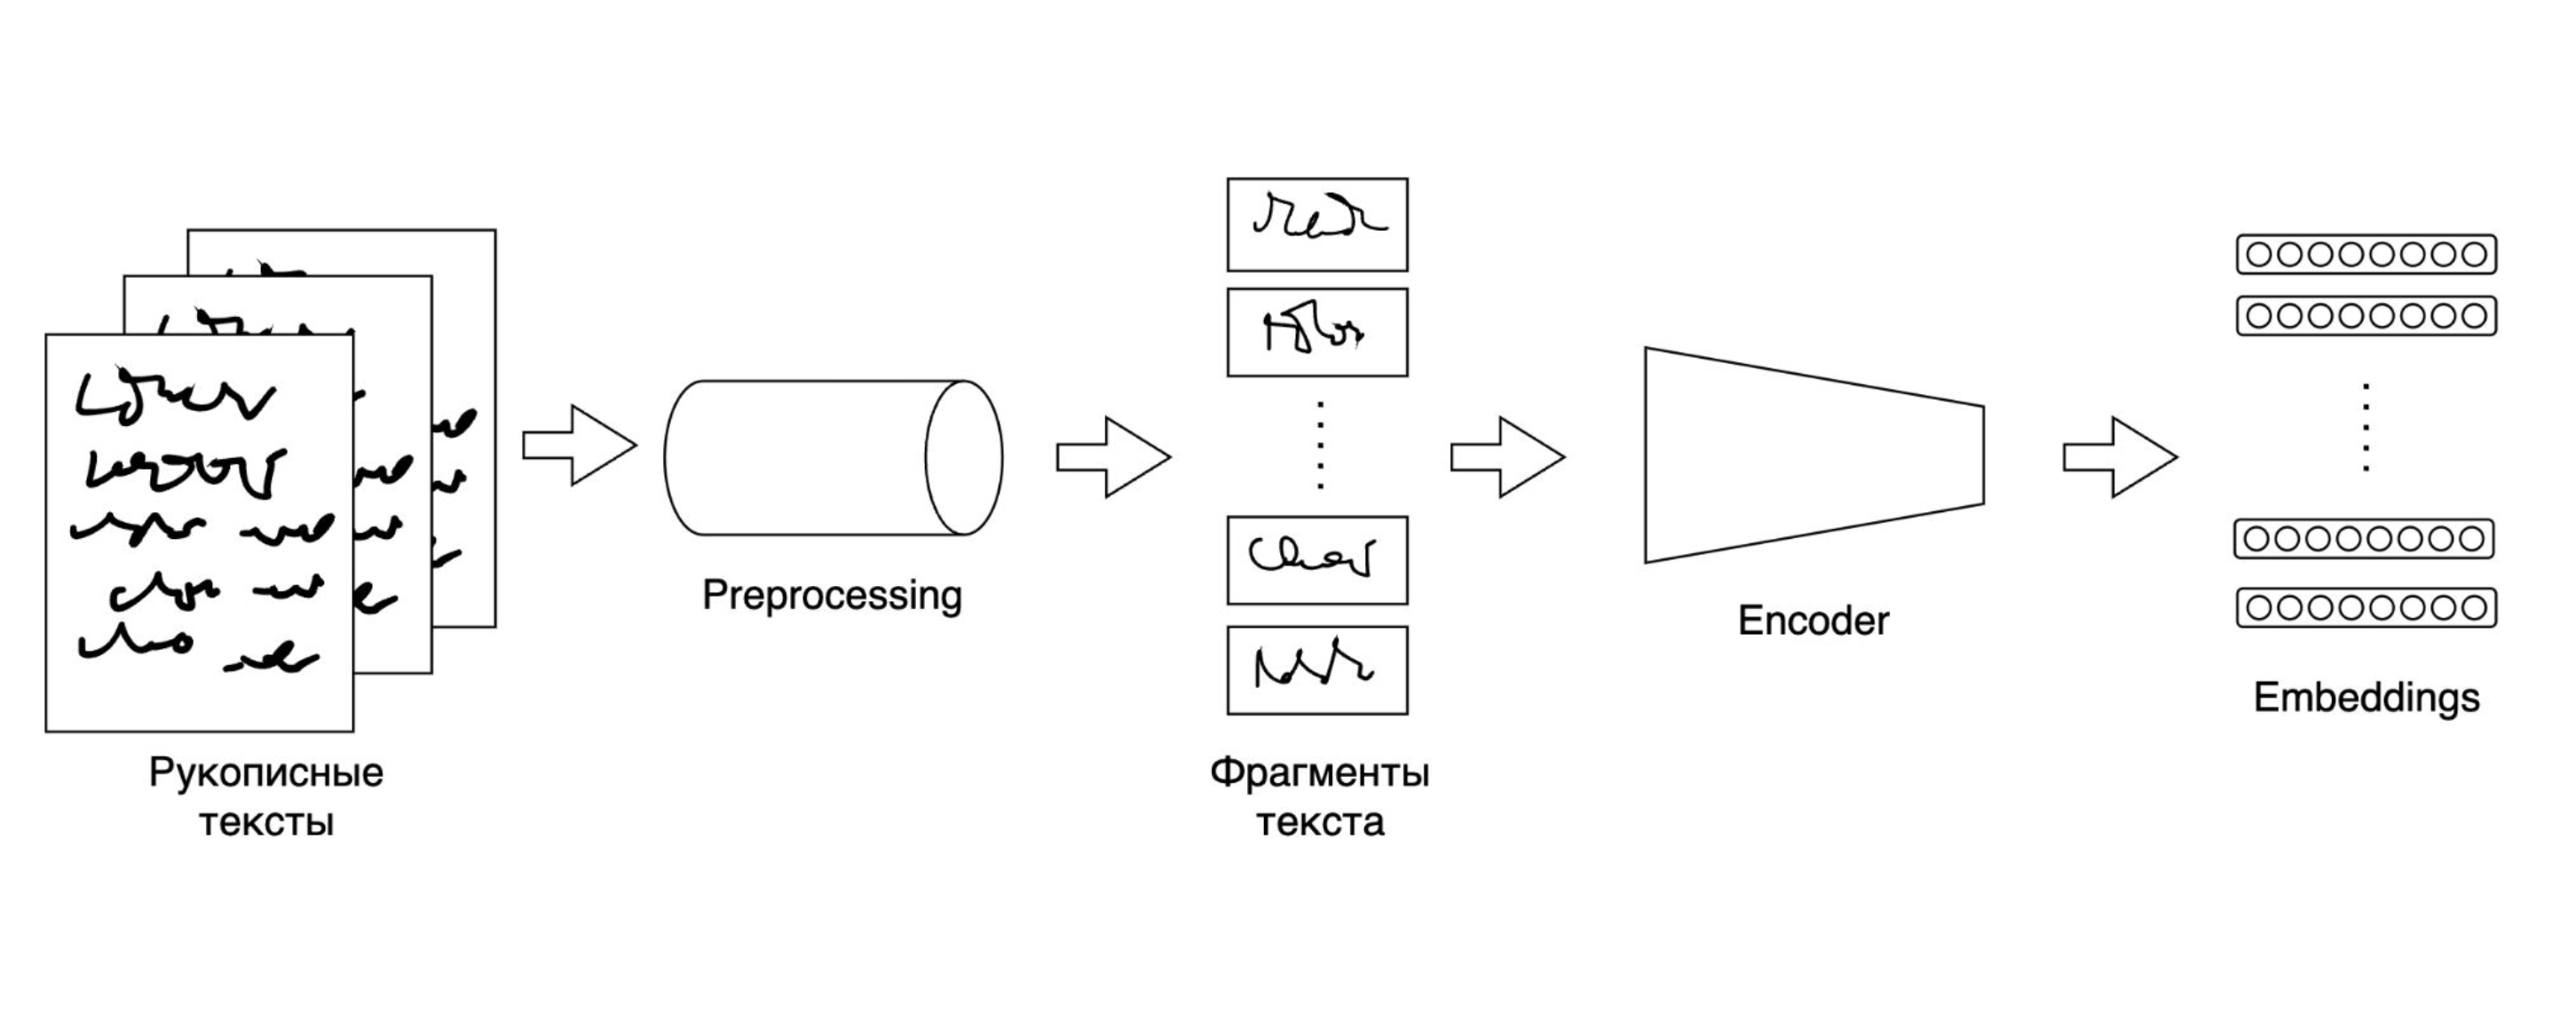
\includegraphics[width=1\textwidth]{5.png}
        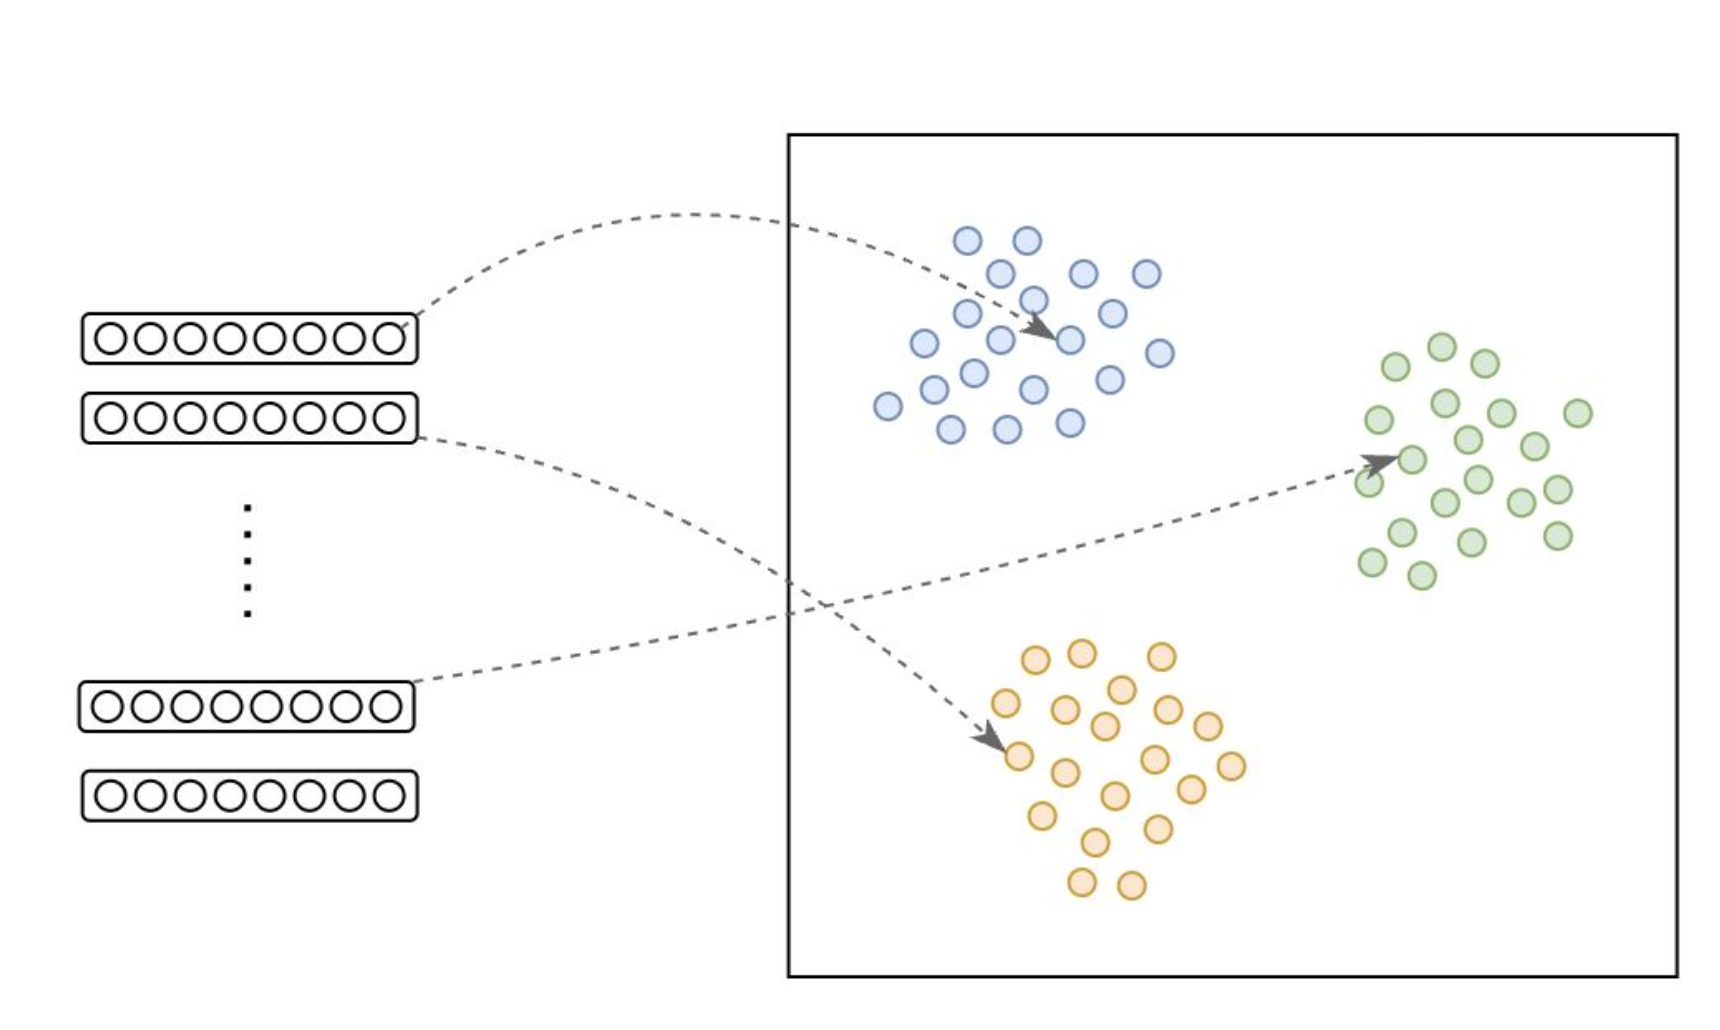
\includegraphics[width=0.8\textwidth]{6.png}
        \caption{Общая архитектура решения задачи кластеризации авторов.}
        \label{fig:general}
    \end{figure}

\subsection{Препроцессинг и агрегирование}

    На вход энкодеру не подается целое изображение документа рукописного текста, так как в нем может содержаться лишняя информация, и энкодеру может быть сложно извлечь репрезентативные признаки из него.

    Одним из самых простых решений этой проблемы является нарезание текста на фрагменты одинаковой ширины. Если учитывать, что высота одной строки текста одинакова, то при обучении сети не придется менять размер фрагментов или применять паддинг, чтобы их объединить в батч, тем самым сохраняя все информацию, содержащуюся во фрагменте, и не допуская смещения модели во время ее обучения. 

\subsubsection{Детекторы углов}

    Однако даже в уже нарезанном фрагменте может содержаться лишняя информация, так как прямые линии, содержащиеся в почерке, и пустые элементы на бумаге не содержат много информации, по которой можно различить автора. В связи с этим можно энкодеру подавать только фрагменты, содержащие самую важную информацию, например, углы и пересечения. Найти подобные участки могут помочь так называемые детекторы углов. Существует множество алгоритмов в данной области. Самыми классическими являются Harris \cite{harris} и FAST \cite{fast}.

    \paragraph{Harris Corner Detector}\mbox{} \\
    Главная идея детектора Харриса заключается в том, что при сдвиге какого-то окна с угла в любом направлении сильно изменится контент самого окна. Чтобы это формализовать, введем обозначения. Пусть $I$ -- исходное изображение, $W$ -- какое то окно, $\Delta x$ и $\Delta y$ -- направление смещения окна. Тогда $E$ -- разница при смещении окна -- вычисляется по этой формуле:

    $$
    E \; = \sum_{(x, y) \in W} \left( I(x, y) - I(x + \Delta x, y + \Delta y)\right)^2
    $$
    \smallskip
    \noindent

    При разложении в ряд Тейлора, вышеописанная сумма может быть представлена в матричной форме:

    $$
    E \; \approx \begin{pmatrix}
        \Delta x & \Delta y
        \end{pmatrix} 
        M\begin{pmatrix}
        \Delta x\\
        \Delta y
        \end{pmatrix}
    $$

    \smallskip
    \noindent
    где $M$ -- матрица следующего вида:

    $$
    M = \begin{pmatrix}
        \sum_{(x, y) \in W} I^2_x & \sum_{(x, y) \in W} I_x I_y \\
        \sum_{(x, y) \in W} I_x I_y & \sum_{(x, y) \in W} I^2_y \\
    \end{pmatrix}
    $$

    \bigskip
    \noindent

    Таким образом, значение изменения контента напрямую зависит от матрицы $M$, и нам достаточно работать именно с ней. Чтобы определить с помощью матрицы $M$, если ли действительно угол в окне, применяется следующий индикатор:
    $$
        R = \det(M) - k \: \text{tr}(M)^2
    $$
    \noindent

    Последнюю формулу можно переписать с помощью собственных значений матрицы $M$:

    $$
        R = \lambda_1 \cdot \lambda_2 - k \: (\lambda_1 + \lambda_2)^2
    $$
    \noindent

    Обычно $k$ берут из отрезка $[0.04; 0.06]$. Если значения $R$ положительные и достаточно большие, то мы нашли угол. 

    \paragraph{FAST Corner Detector}\mbox{} \\

    Данный метод берет более алгоритмический подход к нахождению углов, чем метод Харриса. Для фиксированной точки берется окружность радиуса 3, которая состоит из 16ти пикселей, пронумерованных по часовой стрелке начиная с 12ти часов. Если какая-то непрерывная последовательность $N$ точек ярче/темнее зафиксированного центра окружности на какую-то величину, то мы можем сказать, что нашли угол. 

    \begin{figure}[htbp]
        \centering
        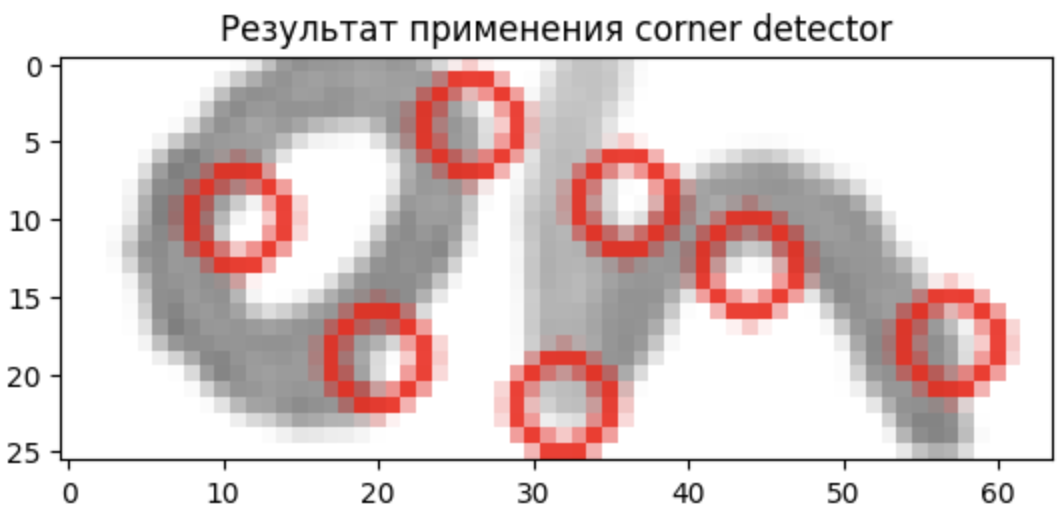
\includegraphics[width=0.7\textwidth]{11.png}
        \caption{Пример применения детектора углов FAST на вырезанном слове из датасета CVL. Как можно заметить, он обнаруживает углы и пересечения, которые содержат максимальную информацию о почерке. Далее при обучении извлекаются фрагменты в этих местах определённого размера и подается в энкодер.}
        \label{fig:fast_example}
    \end{figure}

    При этом может быть вычислительно дорого проверять данное условие для каждого пикселя. Поэтому перед этим проверяют немного оптимизированное условие, путем того, что смотрят на 1й, 5й, 9й и 13й пиксели. Как минимум три из них должны быть ярче или темнее зафиксированного центра. Если это не так, то нет смысла проверять все пиксели.

    Данный метод показал хорошую точность и результаты скорости работы по сравнению с Harris Corner Detector.

\subsubsection{Агрегирование локальных фрагментов: VLAD}

    После того, как энкодер обработал куски рукописного текста, на выходе мы имеем множество локальных эмбеддингов. Существует несколько способов получения глобального вектора, содержащего репрезентативные признаки текста. 

    Одним из алгоритмов является VLAD: Vector of Locally Aggregated Descriptors \cite{vlad_original}. Данный алгоритм позволяет получить из локальных дескрипторов общий глобальный вектор фиксированного размера, который содержит достаточно информации для идентификации изображения. Сначала формируется словарь визуальных слов $C = \{ c_1, \dots, c_k \}$ фиксированного размера $k$ с помощью алгоритма кластеризации K-Means, где $k \in \mathbb{R}$ -- гиперпараметр. Затем каждому локальному дескриптору $x_i$ сопоставляется ближайшее визуальное слово. Наконец, глобальный эмбеддинг $v \in \mathbb{R}^{k \times d}$ вычисляется по данной формуле:
    $$
        v_{i, j} = \sum_{x \text{ ближайшие к } c_i} (x_j - c_{i, j}) = \sum_{i = 1}^N a_k(x_i) \cdot (x_i - c_{i, j})
    $$

    \noindent
    где $d$ -- размерность пространства локальных эмбеддингов.

    Однако, недостатком такого метода является его недифференцируемость. Его нельзя сделать частью модели, которая будет обучаться на картинках рукописных текстах. Таким образом, во время обучения мы не можем обучить именно глобальные эмбеддинги, и мы должно будем полагаться на алгоритм VLAD, чтобы он дал глобальные вектора, обладающие нужными нам геометрическими свойствами кластеризуемости.
    
    \begin{figure}[htbp]
        \centering
        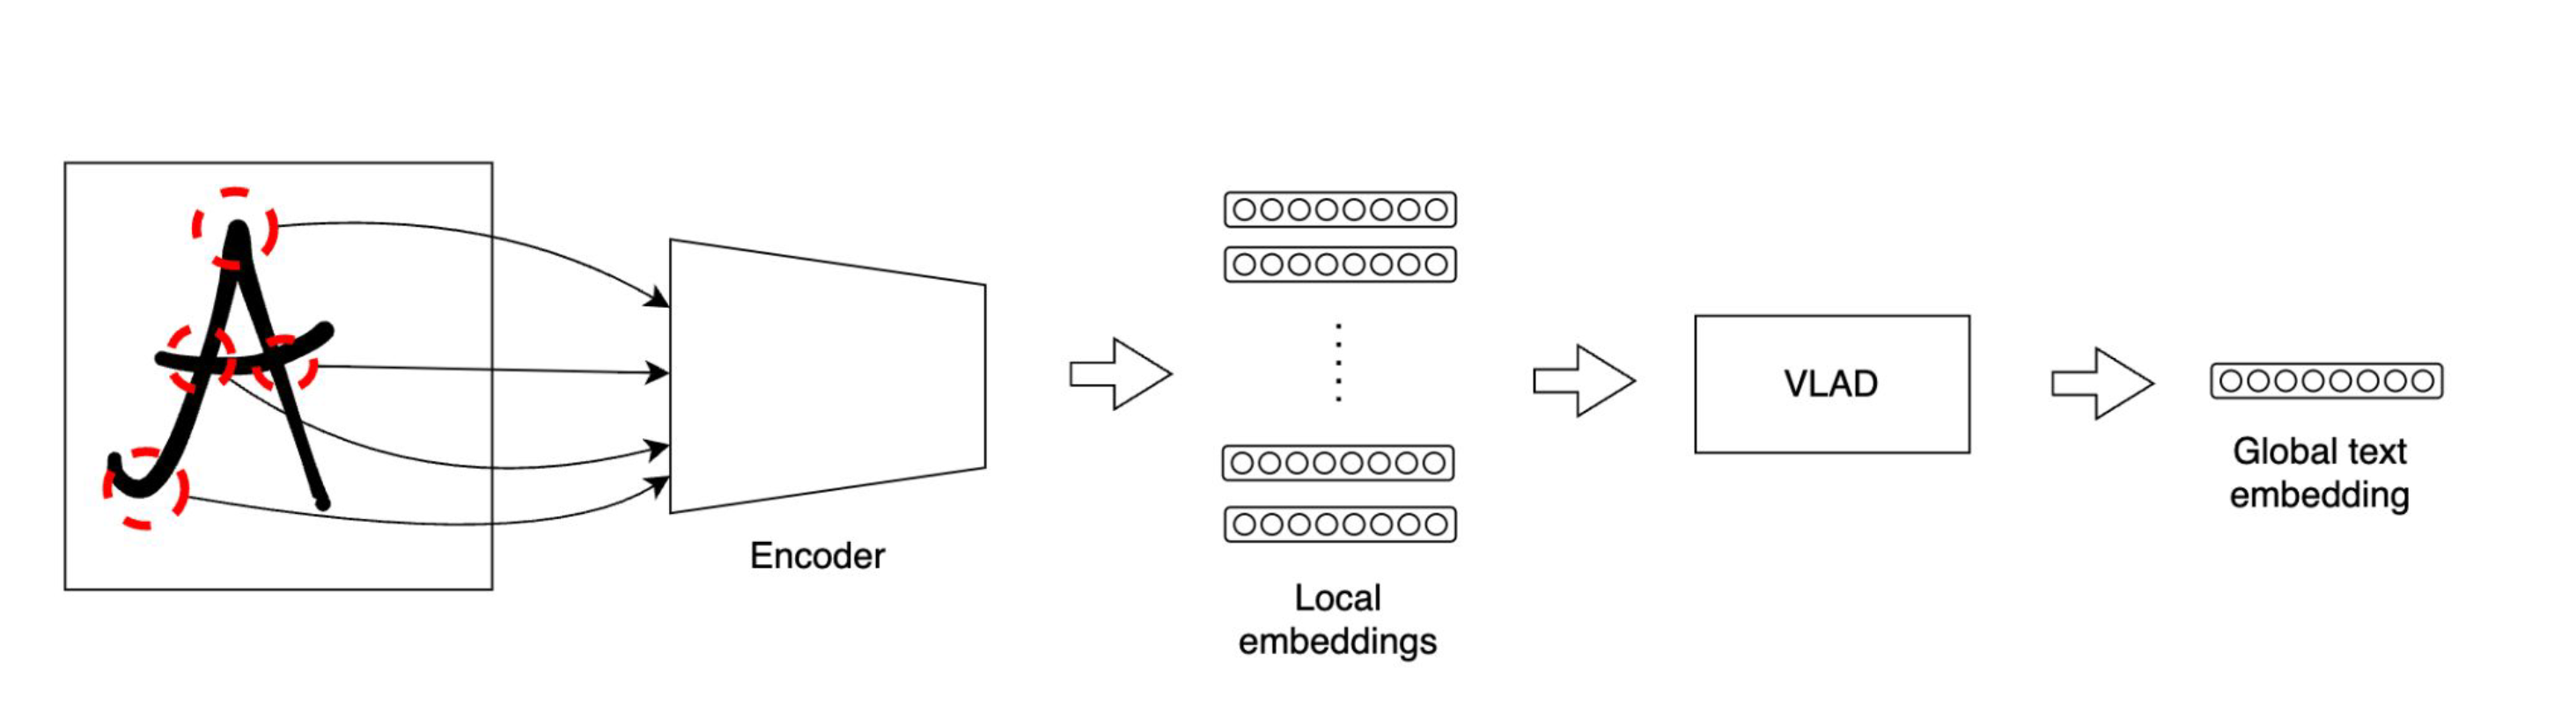
\includegraphics[width=1\textwidth]{1.png}
        \caption{Архитектура c использованием corner detector и VLAD.}
        \label{fig:corner}
    \end{figure}

    Для решения проблемы существует обновленная версия данного алгоритма, называемая NetVLAD \cite{netvlad}. Она представляет из себя слой, который сопоставим с любой свёрточной нейронной сетью, полученный путем замены недифференцируемой операции соотношения локальных дескрипторов визуальным словам на \textit{мягкое} присваивание сразу нескольким кластерам:
    
    $$
        a_k(x_i) = \frac{e^{- \alpha || x_i - c_k ||^2}}{\sum_{k'} e^{- \alpha || x_i - c_k' ||^2}}
    $$
    \smallskip

    \noindent
    где $\alpha$ -- гиперпараметр, $a_k(x_i) \in (0, 1)$, наибольший вес. При $\alpha \rightarrow + \infty$, \: NetVLAD стремится вести себя аналогично оригинальному алгоритму VLAD.

    С его помощью мы сможем обучать агрегирование локальных эмбеддингов таким образом, чтобы глобальный вектор обладал нужными для нас свойствами, которые помогут нам кластеризовать по авторам более точно. Таких свойств мы уже будет добиваться на этапе обучения энкодера.

\subsection{Обучение энкодера}

    Мы поняли как подать свёрточной нейронной сети изображение, чтобы на выходе получить вектор. Но теперь нужно обучить энкодер выдавать именно репрезентативные и кластеризуемые эмбеддинги. Для этого существует несколько способов, которые будут описаны далее.

\subsubsection{Auto-encoder}

    \begin{figure}[htbp]
        \centering
        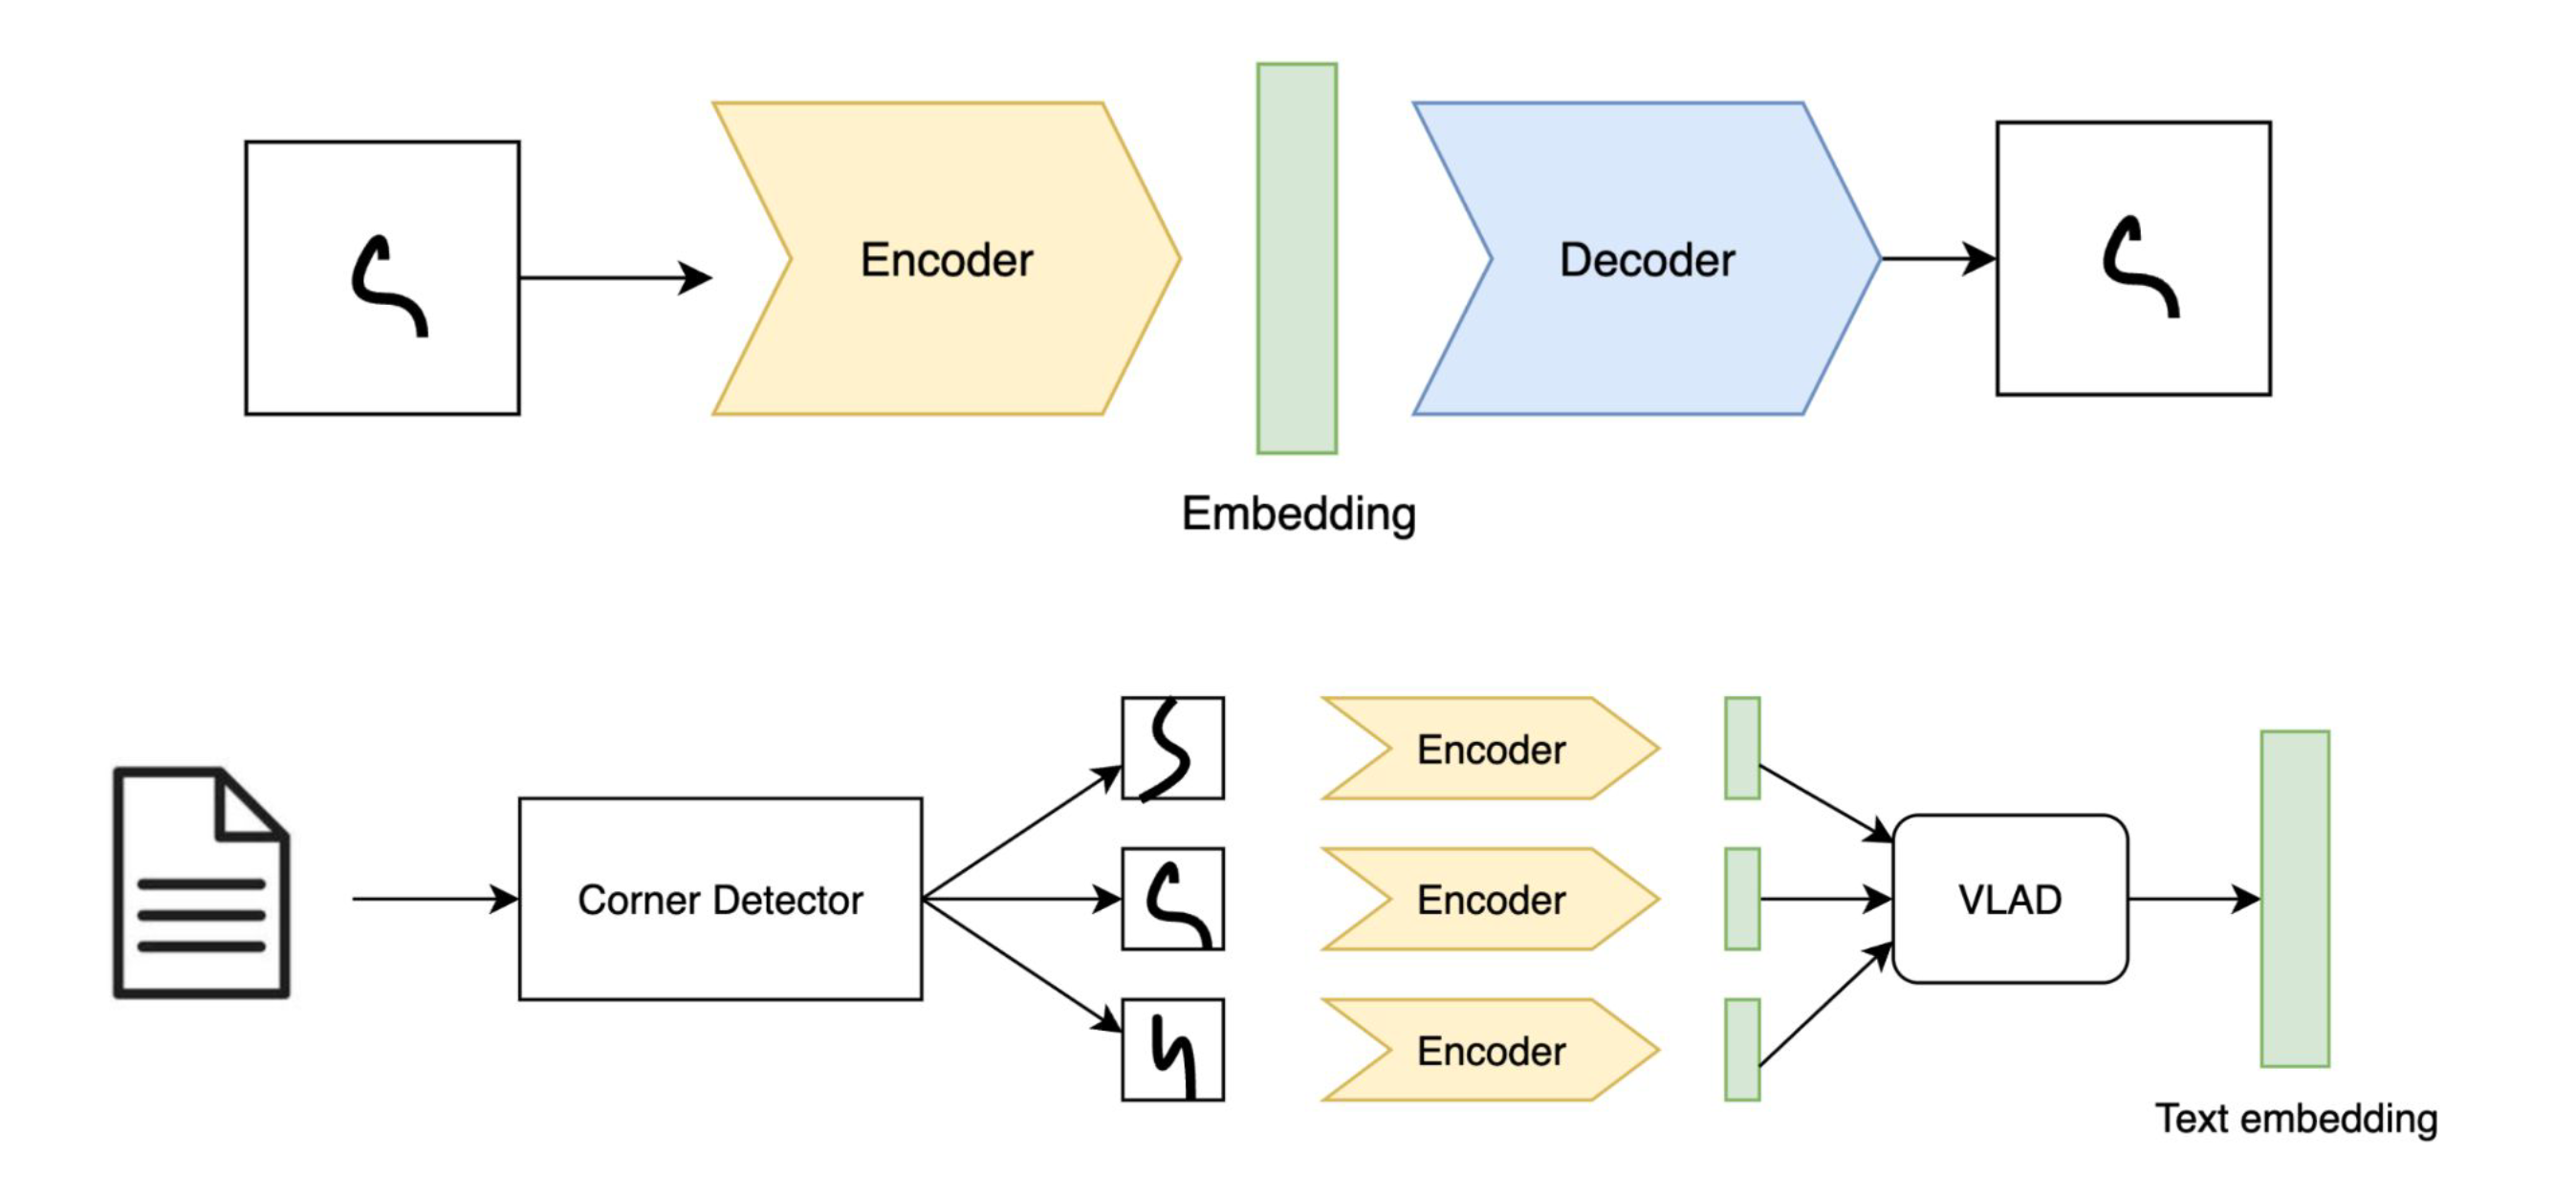
\includegraphics[width=1\textwidth]{7.png}
        \caption{Архитектура автоэнкодера.}
        \label{fig:autoencoder}
    \end{figure}

    Во время выполнения данной работы мы хотели добиться минимального использования меток авторов во время обучения модели. Использование архитектуры автоэнкодера является одним из самых простых способов получения данного результата. Автоэнкодер представляет из себя комбинацию двух свёрточных нейронных сетей, одна из которых называется энкодером, а вторая декодером. Данная архитектура обучается на задаче восстановления изображения, которое подается в начале модели. Предполагается, что после обучения энкодер научится "сжимать" подаваемое на вход изображение в промежуточное состояние, представленное в виде вектора определенной размерности, таком образом, чтобы имеющийся декодер умел уже восстанавливать исходное изображение. Соответственно, промежуточное состояние содержит достаточно информации для восстановления изображения, и, в силу гладкости нейронной сети как обычной математической функции, можно построить гипотезу, что эмбеддинги одинаковых почерков должны находится близко друг к другу. 

\subsubsection{Сиамская нейронная сеть}

    \begin{figure}[htbp]
        \centering
        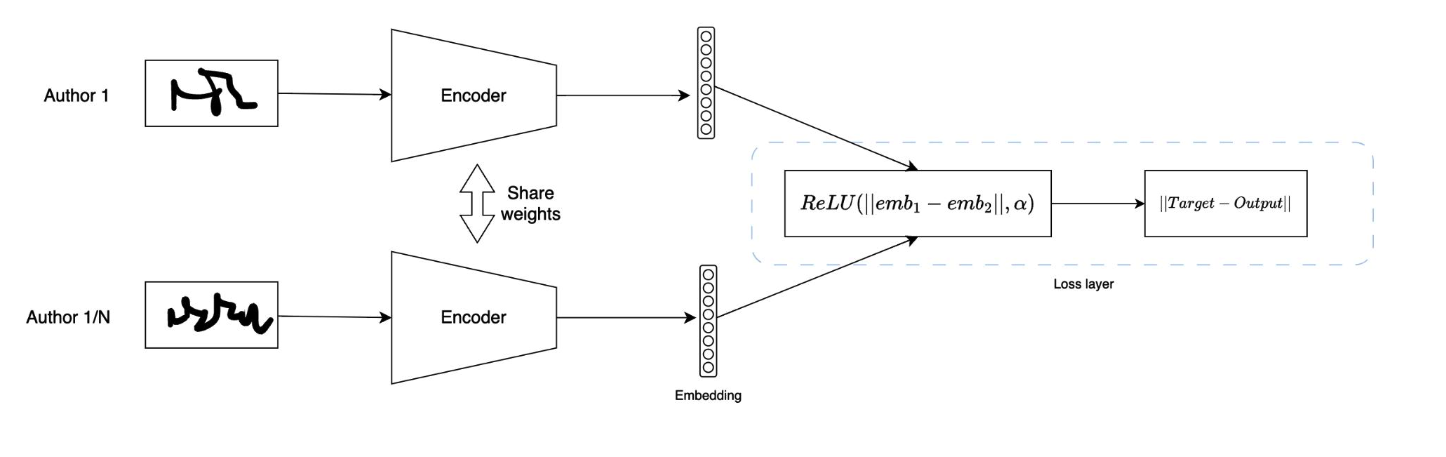
\includegraphics[width=1\textwidth]{2.png}
        \caption{Архитектура Сиамской нейронной сети.}
        \label{fig:snn}
    \end{figure}

    Другая идея обучения энкодера исходит из того факта, что мы хотим получить именно кластеризуемые эмбеддинги. Это значит, что эмбеддинги текстов одного автора должны находиться на максимально близком расстоянии, а эмбеддинги различных авторов -- на далеком, чтобы потом алгоритм кластеризации смог отделить "облака" векторов. Существует множество методов обучения нейронных сетей, которые непосредственно закладывают вышеописанное свойство в процесс обучения. Одним из таким методов является архитектура сиамской нейронной сети (SNN). Она представляет из себя пару идентичных нейронных сетей, веса которых непосредственно связаны. Во время обучения подаются пары изображений как от одного автора, так и от разных авторов. Сеть обучается таким образом, чтобы определенная заранее метрика между векторами текстов от одного автора была минимальна, а между векторами от разных авторов -- как минимум равнялась какому-то гиперпараметру $\alpha$. 

    Определим функцию потерь для данной сети следующим образом. Пусть
$x_i$, $x_j$ -- изображения почерка, которые подаются SNN на вход, $c_k$ -- множество изображений от автора с номером $k$, $\alpha$ -- числовой гиперпараметр. Функцией отсечения назовем: 
$$
    \text{ReLU}(y, \alpha) = 
\begin{cases}
    y,& 0 \le y < \alpha \\
    \alpha,& y \geq \alpha
\end{cases}
$$

\bigbreak
\noindent
Она будет использоваться в формуле функции потерь. Мы не хотим наказывать нейронную сеть во время обучения за то, что эмбеддинги находятся слишком далеко. Поэтому если расстояние между ними будет больше $\alpha$, то мы будем отсекать его по заранее заданному гиперпараметру. 

\begin{figure}[htbp]
    \centering
    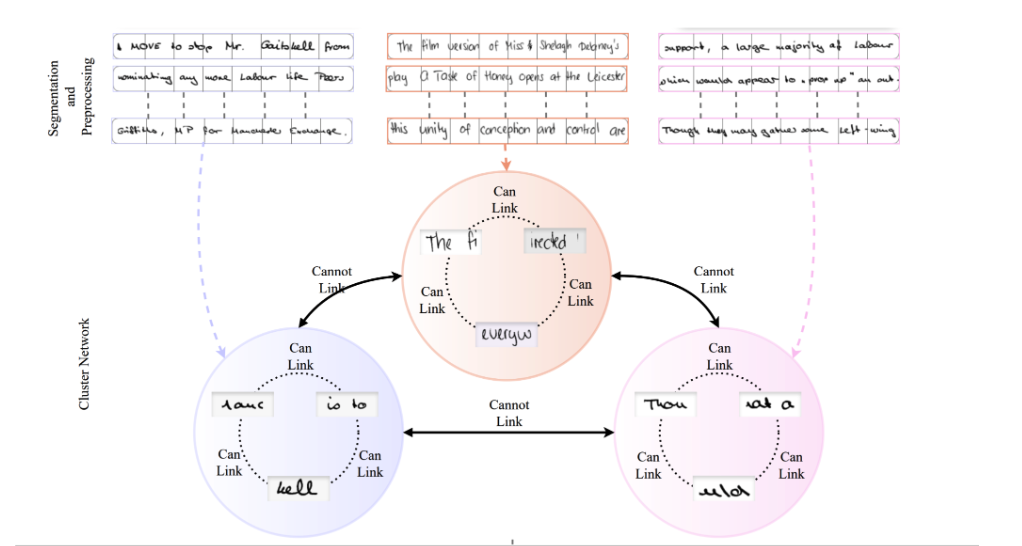
\includegraphics[width=0.8\textwidth]{14.png}
    \caption{Формальное описание кластеров, получаемых в результате работы SNN \cite{snn}. Пусть у нас есть фрагмент $x$ и фрагмент $y$. Мы говорим, что оба фрагмента \textit{стыкуются} (can link), если они взяты от одного автора, и \textit{не стыкуются} (cannot link), если они были написаны разными людьми. Заметим, что в данном определении мы не обращаем внимание на то, что куски в результате стыковки образуют осмысленное слово, так как нам не важен контент, а именно почерк человека.}
    \label{fig:autoencoder}
\end{figure}

\noindent
Определим целевую функцию:
$$
Target =
\begin{cases}
    0,& x_i, x_j \in c_k \\
    \alpha,& x_i \in c_k \text{ and } x_j \in c_q
\end{cases}
$$
Если изображения принадлежат одному автору (находятся в одном множестве $c_k$), то расстояние между ними должно быть равно нулю. Иначе, если они от разных авторов, то расстояние должно быть как минимум $\alpha$. 

\noindent
Наконец, определим функцию потерь:
$$\text{Loss}(Target, emb_1, emb_2) = ||\text{ReLU}(|| emb_1 - emb_2 ||, \alpha) - Target||$$

\noindent
Как мы видим, перед тем как сравнивать расстояние между эмбеддингами и значение target, мы производим отсечку, чтобы не наказывать сеть за слишком далекие друг от друга эмбеддинги.

\subsubsection{Обучение на задаче классификации}

Альтернативной идеей обучения энкодера является обучение его на задаче классификации, с последующим отсечением классификатора. Стандартной архитектурой при обучении на задаче классификации является связка свёрточной и полносвязной нейронных сетей. Можно простроить гипотезу, что эмбеддинги, которые выдает энкодер во время обучения, обладают геометрическими свойствами, которые позволяют классификатору понять к какому автору рукописный текст действительно относится.

Функция потерь в данной ситуации играет огромную роль, так как именно от нее зависит каким образом полученные эмбеддинги будут расположены в пространстве. Обычно при обучении классификатора применяют стандартную функцию SoftMax:

$$
L_{\text{SM}} = -\text{log} \frac{e^{W_{y_i}^T x_i + b_{y_i}}}{\sum_{j=1}^{N} e^{W_{j}^T x_i + b_{j}}},
$$
\smallskip

\noindent
где $x_i \in \mathbb{R}^d$ -- эмбеддинг $i$-го изображения от автора с номером $y_i$, $d$ -- размерность пространства эмбеддингов, $W$ и $b$ задают линейное преобразование. Однако, данная функция потерь никак не способствует близости эмбеддингов от одного автора и дальности эмбеддингов из разных классов, и при большом количестве авторов пространство векторов будет плохо кластеризуемо \cite{arcface}. 

Поэтому в области распознавания лиц используют другую функцию потерь для задачи классификации \cite{arcface}. 

$$
L_{\text{ArcFace}} = - \text{log} \frac{e^{s\:\text{cos}(\theta_{y_i} + m)}}
{e^{s\:\text{cos}(\theta_{y_i} + m)} + \sum^{N}_{j=1, j \neq y_i} e^{s\:\text{cos}(\theta_j)}}
$$
\smallskip

При обучении с функцией потерь ArcFace эмбеддинги распространяются по гиперсфере радиуса $s$, и меняется именно угловое расстояние между ними. При этом обеспечивается интервал с геодезическим расстоянием $m$ между эмбеддингами разных классов. Это свойство может дать хорошо кластеризуемые вектора.

\begin{figure}[htbp]
    \centering
    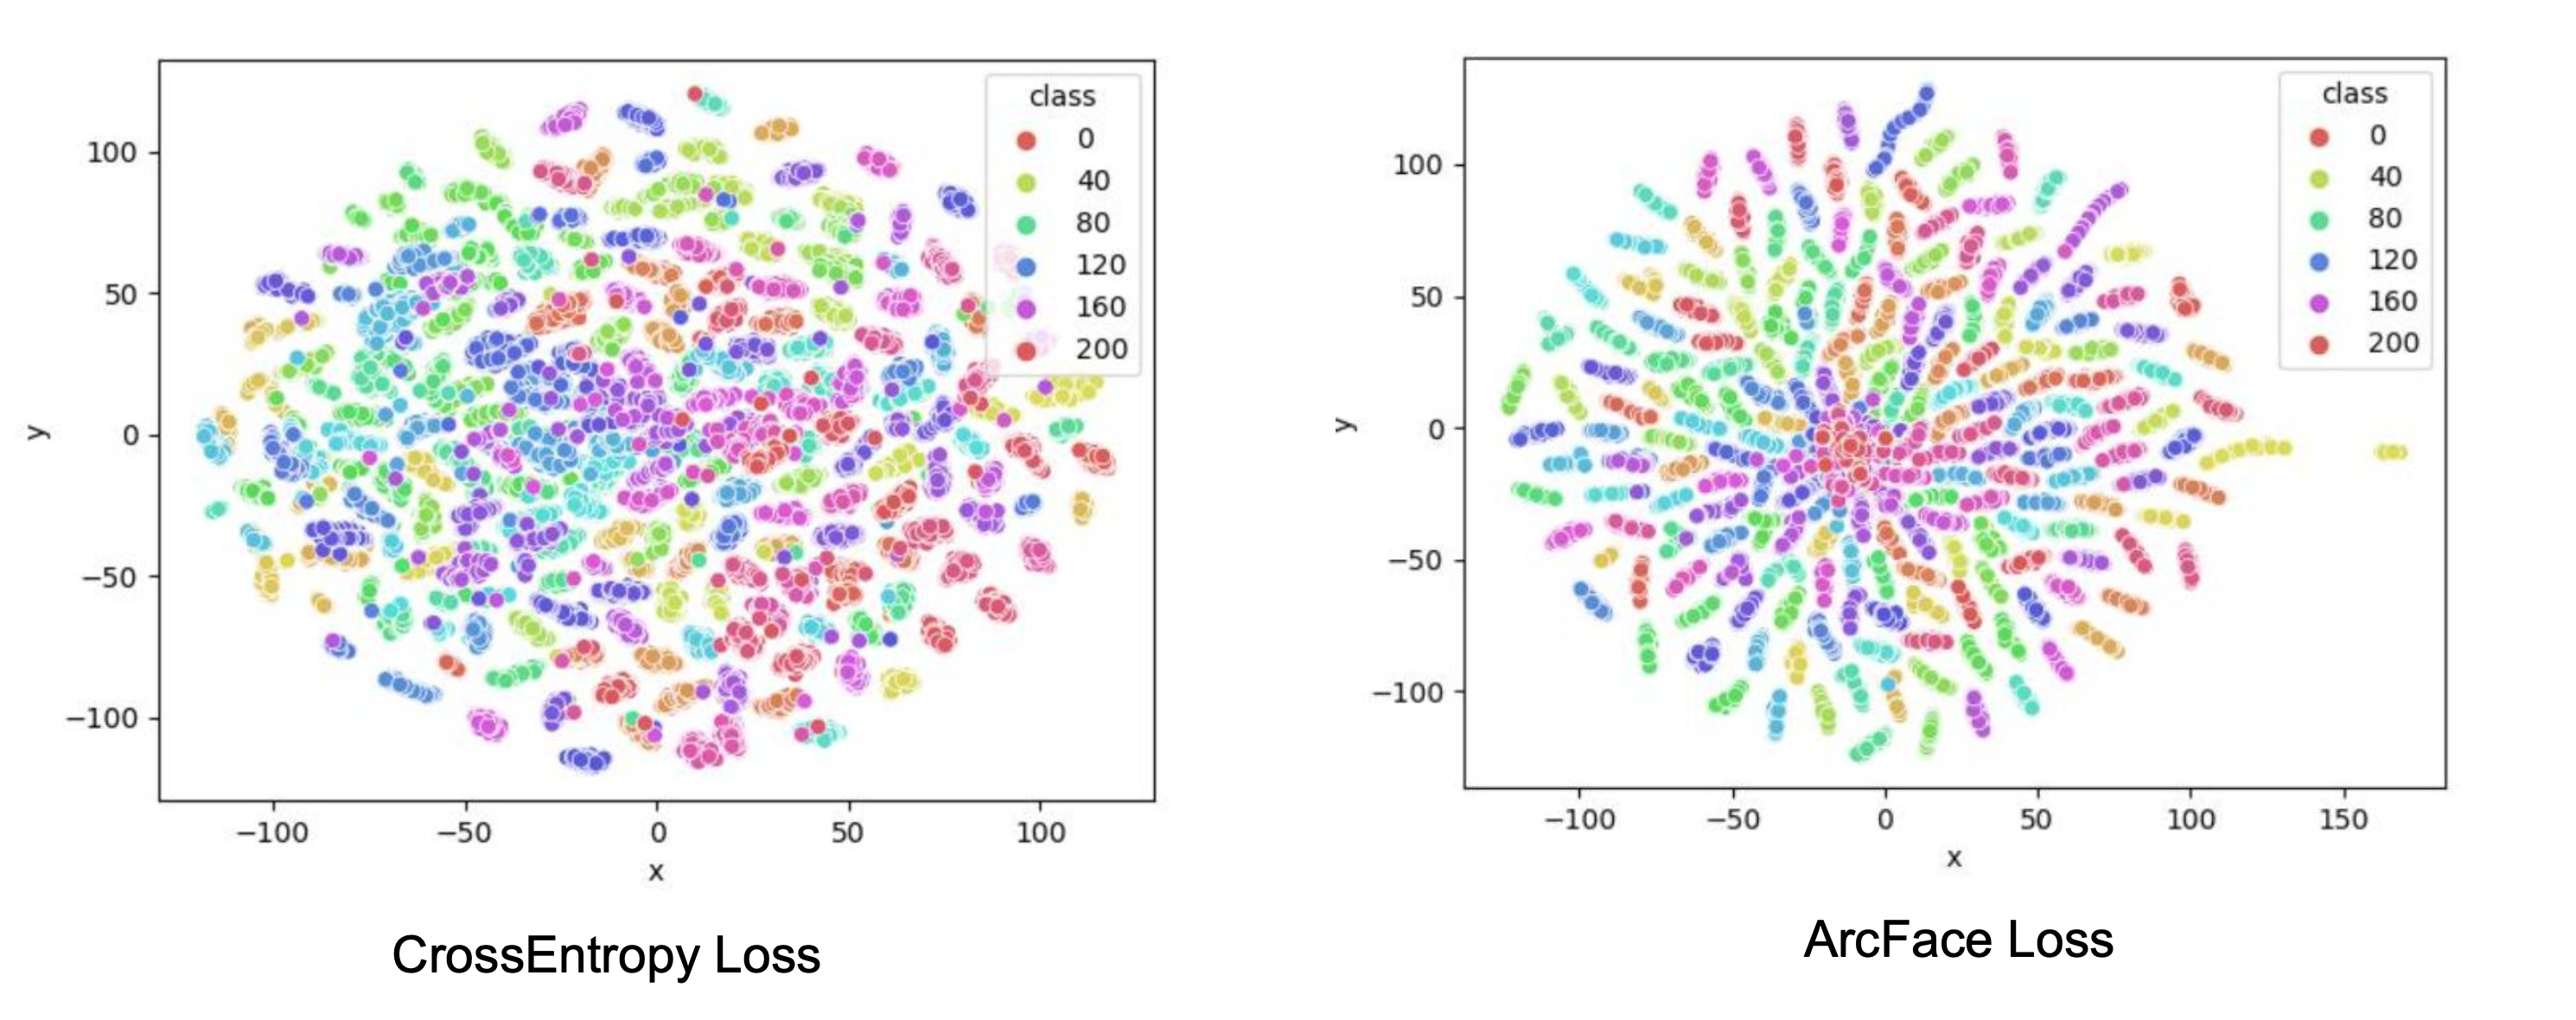
\includegraphics[width=1\textwidth]{4.png}
    \captionsetup{width=0.9\textwidth}
    \caption{Результат применения T-SNE к обученным эмбеддингам в рамках задачи классификации. На левом графике модель обучалась с функцией потерь CrossEntropy Loss. На правом графике -- с ArcFace. Как мы видим, кластера точек на правом графике более различимы. Более того, они образуют некоторые кривые, так как в оригинально пространстве находятся на $n$-мерной сфере.}
    \label{fig:ce_vs_arcface}
\end{figure}

Кроме этого, хорошие результаты в области распознавания изображений продемонстрировал Triplet Loss \cite{triplet_loss}\cite{netvlad}. Данная функция потерь помогает обучить хорошие эмбеддинги таким образом, чтобы они были также легко отделяемыми. Для этого во время обучения выделяют три изображения: Anchor -- якорь, Positive -- положительное изображение, которое находится в одном классе с якорем, Negative -- негативное изображение из другого класса. Цель Triplet Loss заключается в том, что два примера из одного класса находились как можно ближе друг к другу, а из разных классов -- как можно дальше. Функция потерь определяется следующим образом:

$$
L_{\text{Triplet}} = \max(m(a, p) - m(a, n) + \text{margin}, 0)
$$

\noindent
где $m$ -- модель, которая выдает эмбеддинги, $a$ -- anchor изображение, $p$ -- positive изображение, $n$ -- negative изображение, $\text{margin} \in \mathbb{R}$ -- гиперпараметр, чтобы кластера слишком сильно не схлопывались в точку.

Однако данная постановка определения лосса требует на вход тройку изображений с определенными свойствами. Существует несколько техник, которые позволяют из датасета при обучении получить нужные тройки \cite{tiplet_online}.

\paragraph{Offline triplet mining}\mbox{} \\

Оффлайновый выбор троек подразумевает под собой довольно простой механизм: перед каждой эпохой получать эмбеддинги изображений, потом выделять нужные тройки и прогонять через лосс. Под нужными тройками подразумеваются такие тройки, в которых негативное изображение находится ближе к якорю, чем положительное. Однако такой метод не эффективен с точки зрения вычислений.

\paragraph{Online triplet mining}\mbox{} \\

В онлайн методе мы выбираем тройки из батчей во время обучения. Тройку изображений $(a, b, c)$ будем называть валидной, если $a$ и $b$ принадлежат одному классу, а $c$ -- другому. Тогда остается найти валидные тройки, посчитать и агрегировать лосс по ним. Это можно сделать, используя разные стратегии. Например, можно выбрать все валидные тройки и просто взять среднее от Triplet Loss по ним. Или же среди них выбрать самый худший случай, в котором негативное изображение ближе всего находится к якорю, чем положительное, и посчитать лосс только от него.

\subsection{Синтетический датасет}

\begin{figure}[htbp]
    \centering
    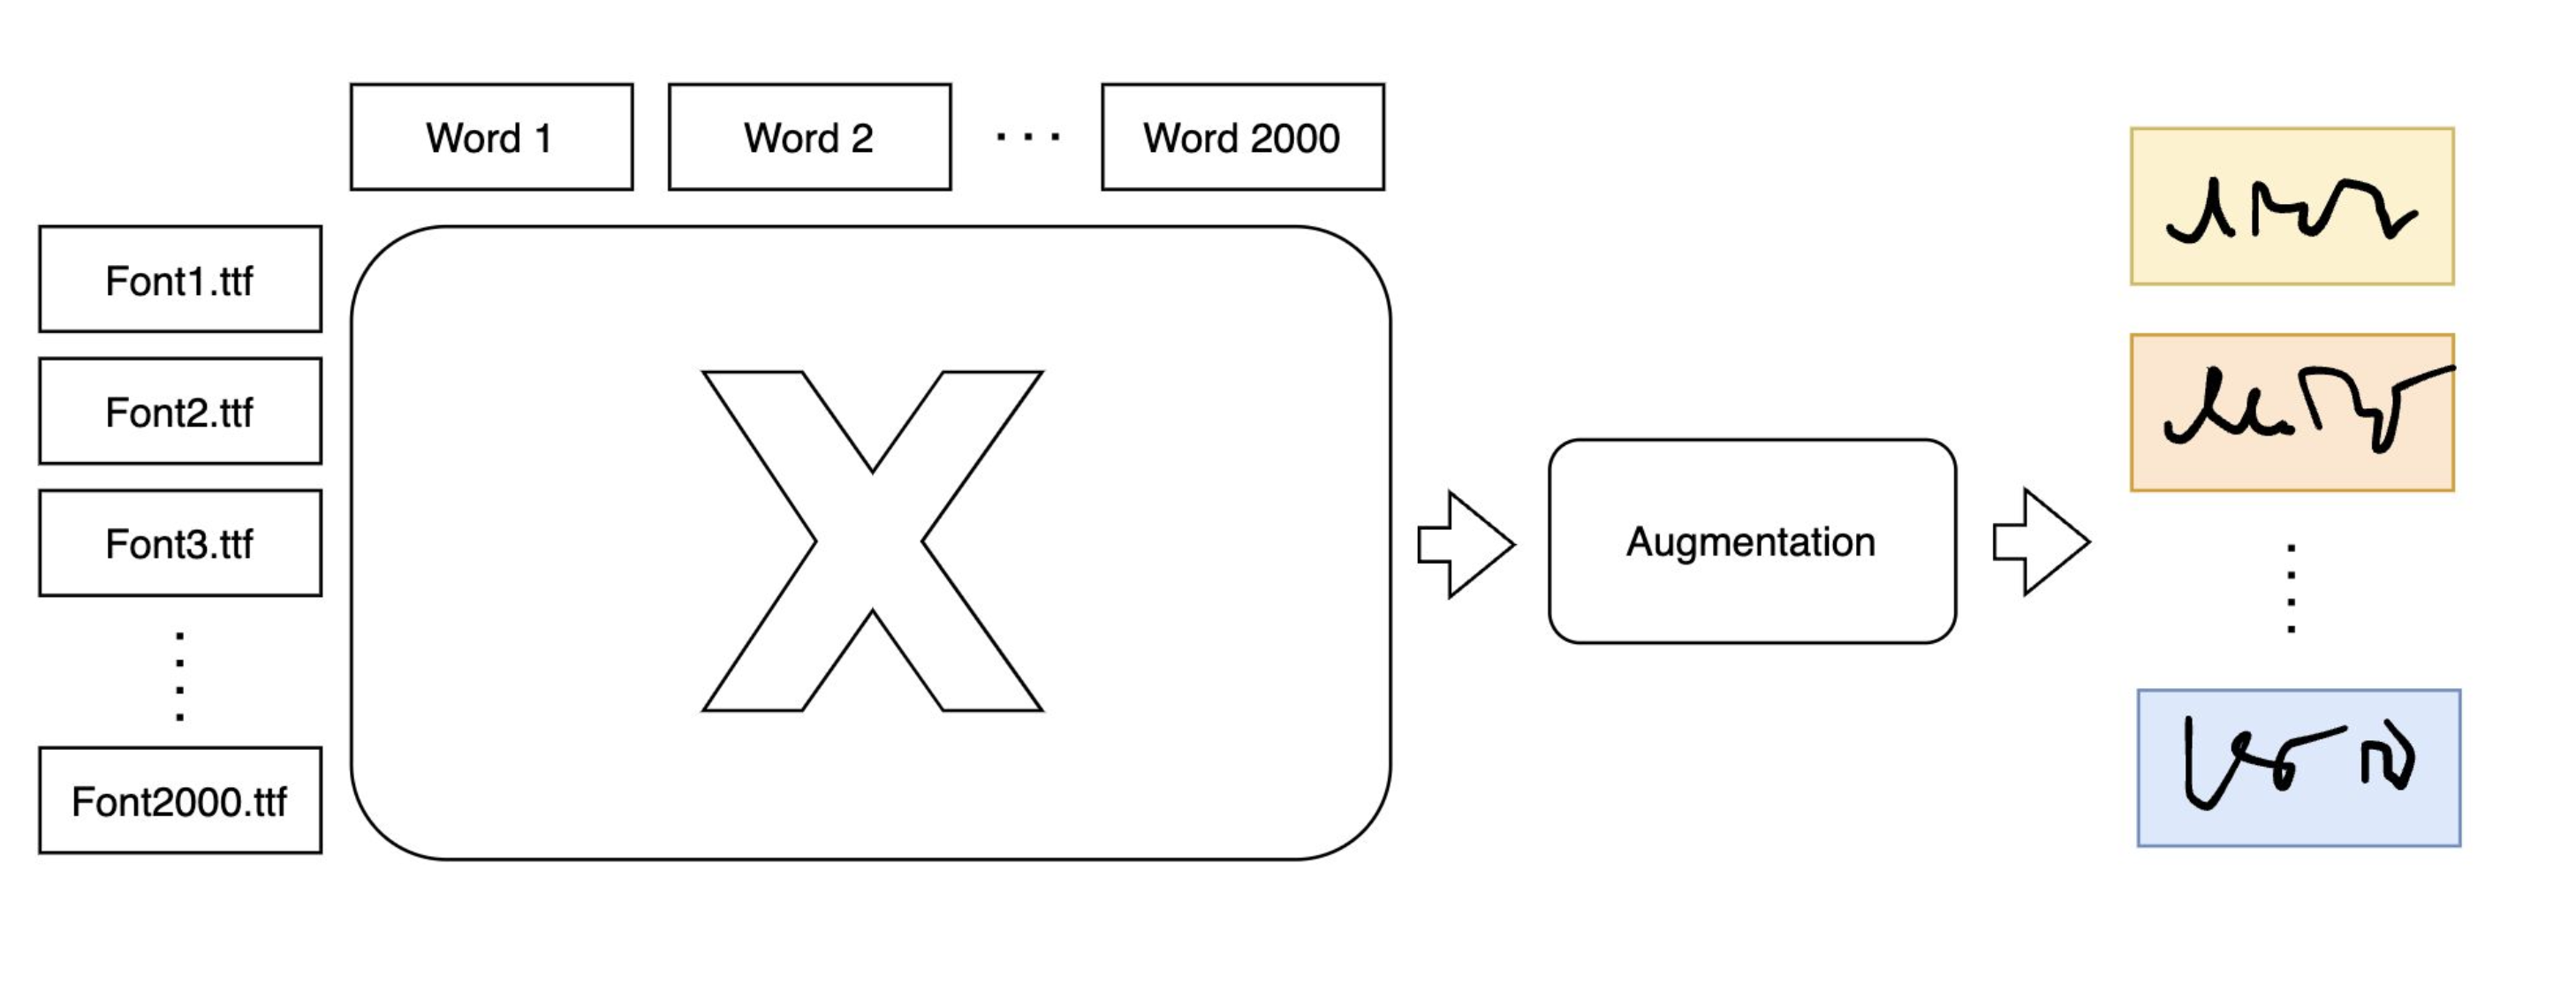
\includegraphics[width=1\textwidth]{3.png}
    \caption{Идея реализации синтетического датасета.}
    \label{fig:synthetic}
\end{figure}

Существует множество датасетов, содержащих рукописные тексты. Самыми популярными из них являются датасеты CVL \cite{cvl} и IAM \cite{iam}. В общей сложности они содержат рукописные тексты от порядка 1000 авторов. Тем не менее, такого количества данных может быть недостаточно для получения хороших результатов обучения крупных свёрточных нейронных сетей из-за проблемы переобучения. 

Есть несколько способов решения этой проблемы. Один из них заключается в аугментации тренировочных данных. Говоря конкретнее, можно изменять текстуру бумаги, силу нажатия и другие параметры почерка, который подается в нейронную сеть для обучения. Таким образом можно уменьшить вероятность переобучения сети.

Но данный способ не решает проблему количества авторов, также как и разнообразности самих почерков. Поэтому существует другой вариант, который подразумевает генерацию самого датасета \cite{font}. Можно отобрать порядка 10000 шрифтов, которые похожи на рукописный текст, применить к ним аугментацию, например, симулировать написание ручкой или чернилами, добавить различных текстур бумаги и освещения, и сгенерировать изображения из 10000 случайных слов английского языка для каждого почерка. Тем самым, мы получим порядка 100 миллионов изображений рукописного текста, что значительно превышает размер натурального датасета.

Данный подход имеет свои преимущества и недостатки. С одной стороны, мы имеем огромное количество данных и классов, что может улучшить качество модели при обучении. С другой стороны, человеческий почерк по своей природе представляет из себя более сложную структуру, так как человек пишет одну и ту же букву в слове немного по разному, в то время как в шрифтах каждая буква будет абсолютно одинаковой. Это может негативно сказаться на качестве обучения.

\begin{figure}[htbp]
    \centering
    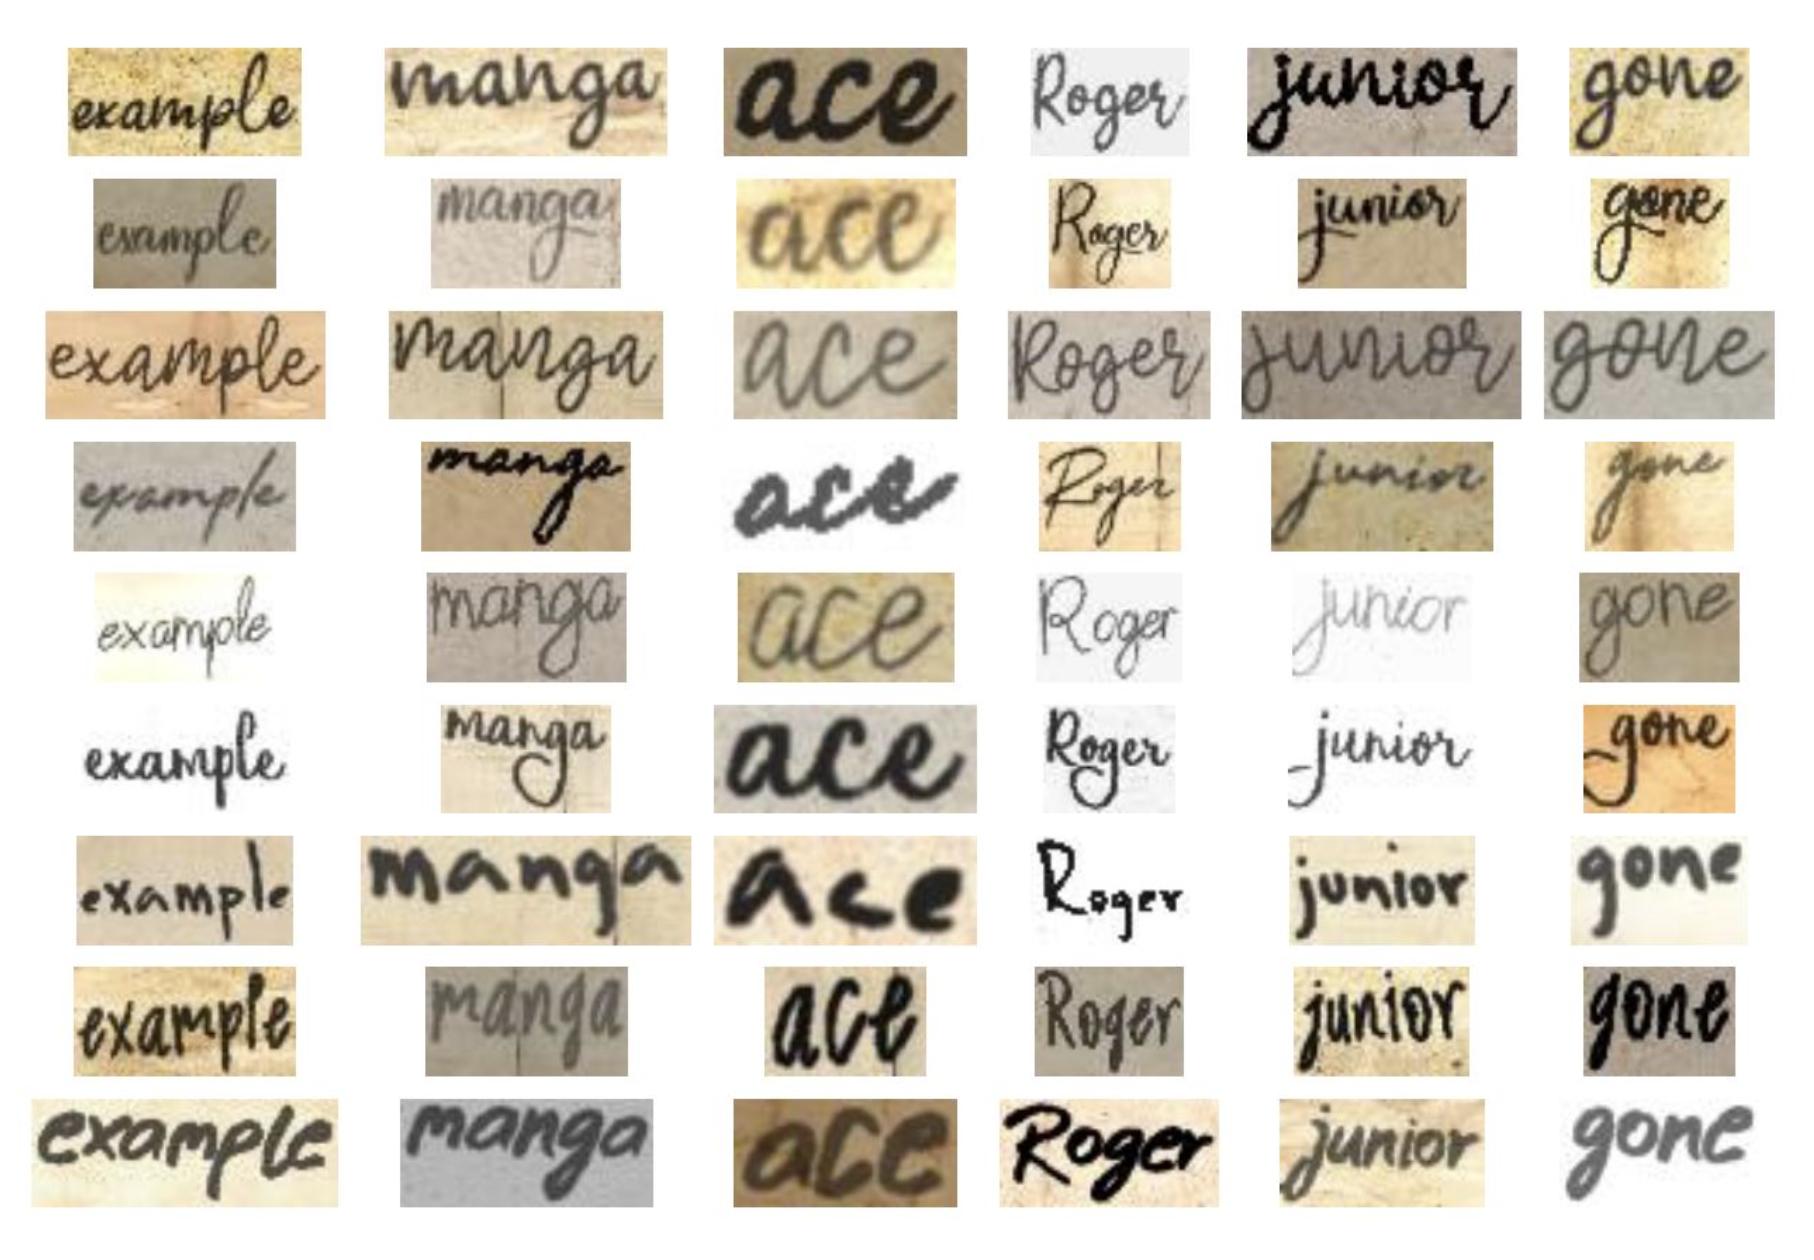
\includegraphics[width=0.7\textwidth]{9.png}
    \captionsetup{width=0.9\textwidth}
    \caption{Результат генерации синтетического датасета \cite{font}. Как можно видеть, искуственно сгенерированные слова довольно похожи на рукописный текст.}
    \label{fig:font}
\end{figure}

\subsection{Уменьшение размерности}

В архитектуре ResNet, которая используется в качестве бэкбоуна практически во всех моделях обучения в данной работе, выходной слой выдает эмбеддинг размерности 512. Проблема заключается в том, что вектора большой размерности довольно плохо поддаются кластеризации. Главной причиной такого явления является феномен \textit{проклятия размерности}. Его можно интерпретировать разными способами. Одна из формулировок является следующей: пусть $n$ векторов из пространства $\mathbb{R}^d$ взяты из некоторого фиксированного распределения. Тогда разница между минимальным и максимальным расстоянием от какой-то фиксированной точки $Q$ до данных точек практически не сравнима с минимальным расстоянием при стремлении размерности пространства к бесконечности \cite{bellman1957dynamic}. Строго говоря:

$$
\lim_{d\rightarrow+\infty} \mathbb{E}\left( 
    \frac{\text{dist}_{\text{max}}(d) - \text{dist}_{\text{min}}(d)}{\text{dist}_{\text{min}}(d)}
\right) = 0
$$

\bigskip
Многие алгоритмы кластеризации используют метрики, которые, в следствии вышеописанного феномена, являются довольно слабыми в многомерных пространствах. В связи с этим есть необходимость в уменьшении размерности пространства эмбеддингов.

Задача уменьшения размерности заключается в том, чтобы построить преобразование, которое переводит пространство векторов в пространство наименьшей размерности, при этом добиваясь наименьших потерь информации и свойств самого пространства. Определение потерь может быть индивидуально для каждого алгоритма. 

Для этого существует несколько подходов. Одним из них является классический метод главных компонент, также известный как PCA. Путем сингулярного разложения матрицы данных, определения главных компонент и проецирования данных на гиперплоскость ортогонально некоторым собственным векторам можно добиться уменьшения размерности с минимальными потерями ковариации. Однако в следствие линейности данного метода, он не всегда дает хорошего результата при значительном уменьшении размерности.

Другим известным алгоритмом является t-SNE. Представляя из себя нелинейный алгоритм уменьшения размерности, он себя хорошо показывает в задаче визуализации многомерных данных. Однако из-за своего устройства он не способен сохранять расстояния между эмбеддингами и также может создавать искусственные кластера. Это хорошо демонстрируют эксперименты его применения на двух облаках точек, взятые из двух независимых гауссовских распределений \cite{pca_bad}.

UMAP является более универсальным алгоритмом уменьшения размерности перед применением алгоритма кластеризации \cite{umap}. В отличии от T-SNE, UMAP сохраняет некоторые геометрические свойства. Он также предоставляет широкий набор параметров, который позволит улучшить качество кластеризации на полученных данных меньшей размерности. Более того, алгоритму можно подать данные c метками, на которых алгоритм может обучиться и выдать более кластеризуемые эмбеддинги.

\subsection{Кластеризация}

Кластеризация является важной частью данной работы. Получив на входе набор эмбеддингов, которые нам дала нейронная сеть и алгоритм уменьшения размерностей, нам нужно теперь выделить кластера рукописных текстов, которые написал один автор. 

Существует огромное количество различных алгоритмов, решающих эту задачу. Каждый из алгоритмов по-своему уникален, имеет собственные параметры, учитывает природу данных также по-разному. 

Более того, довольно важно учитывать саму природу данных, которые мы пытаемся кластеризовать. Принимая в расчет архитектуры, которые были описаны ранее в данной работе, можно прийти к выводу, что как минимум природа эмбеддингов различается в метрике, которая минимизировалась для эмбеддингов от одного автора. Как можно вспомнить, например, модель SNN минимизировала евклидово расстояние между двумя векторами, представляющие рукописные тексты от одного писателя. В то же время, модель, обученная на задаче классификации с функцией потерь ArcFace, будет выдавать эмбеддинги, которые расположены на $n$-мерной гиперсфере и которые обладают свойством кластеризуемости относительно косинусной метрики.

Из вышесказанного следует, что, выбирая алгоритм, важно учитывать специфику данных. На них очень сильно влияет как архитектура нейронной сети, так и выбранный алгоритм уменьшения размерности. 

Хочется отметить два самых главных параметра, которые будут выбираться по-разному в зависимости от выбранной архитектуры модели. Первым является количество кластеров, которое некоторые алгоритмы кластеризации требуют указать заранее. Однако далеко не всегда мы знаем их количество. Более того, в данной работе определение количества авторов является одной из поставленных задач. Тем не менее, существует несколько методик получения количества кластеров, которые будут описаны позже. Вторым важным параметром является непосредственно метрика. Некоторые алгоритмы считают эмбеддинги близкими друг к другу именно благодаря метрике, что является логичным утверждением. Она также будет варьироваться в зависимости от выбранной модели.

\subsubsection{Алгоритмы кластеризации}

Рассмотрим существующие популярные алгоритмы кластеризации.

\paragraph{K-Means}\mbox{} \\

Метод K-Средних является одним из классических алгоритмов кластеризации. Основная задача данного алгоритма заключается в минимизации так называемой \textit{инерции}, что также называется \textit{критерием суммы квадратов внутри кластера}:

$$
\sum_{k=0}^{n} \min_{\mu_j \in C}(||x_i - \mu_j||^2)
$$

\bigskip
\noindent
Данный подход имеет как преимущества, так и недостатки. Из преимуществ можно выделить широкий положительный опыт его использования на различных типах данных, а также масштабируемость данного метода. Он показывает хорошую производительность на большом количестве данных, существует версия MiniBatchKMeans, которая позволяет порциями подавать данные для кластеризации.

Однако, так называемая инерция не является оптимальной метрикой. Как минимум, оно требует нормированности пространства эмбеддингов, так как "растянутые" кластера будут являться контрпримером работы данного алгоритма. Также, алгоритм требует на вход количество кластеров, что для нас является неизвестной величиной, и, возможно, могут появиться трудности с ее определением. Более того, предполагается, что кластера по своей геометрической структуре является выпуклыми множествами относительно зафиксированной метрики. Но при как при обучении наших эмбеддингов, так и при уменьшении размерности, мы это напрямую никак не можем гарантировать, и метод таким образом может показать плохой результат. Также алгоритм плохо себя показывает на векторах высокой размерности, что обусловлено вышеупомянутым феноменом \textit{проклятия размерности}.

\paragraph{Иерархическая кластеризация}\mbox{} \\

Алгоритмы иерархической кластеризации представляют из себя семейство методов, которые объединяет общая идея кластеризации множества векторов путём последовательного слияния и разделения. В начале алгоритма каждый объект находится в собственном кластере. Далее алгоритм находит два самых близких друг к другу кластера и сливает их во едино. Повторяется данный процесс до тех пор, пока не нашлось требуемое количество кластеров.

Данный алгоритм обладает тремя важными параметрами. Первым и вторым, по аналогии с алгоритмом K-Means, являются количество кластеров и метрика соответственно. Третьим параметром подается способ определения расстояния между кластерами. Существует несколько методов для данной задачи. Пусть $U$, $V$ -- кластера точек, $D(U, V)$ -- расстояние между кластерами. Тогда существуют как минимум такие методы \cite{hierarchical}:

\begin{enumerate}
    \item Метод одиночной связи $$D(U, V) = \min(\rho(u, v))$$
    \item Метод полной связи $$D(U, V) = \max(\rho(u, v))$$
    \item Метод средней связи $$D(U, V) = \frac{1}{|U| \cdot |V|}\sum_{u \in U} \sum_{v \in V} \rho(u, v)$$
    \item Метод Уорда $$D(U, V) = \frac{|U| \cdot |V|}{|U| + |V|} \rho^2 \left( \sum_{u \in U} \frac{u}{|U|}, \sum_{v \in V} \frac{v}{|V|} \right)$$
\end{enumerate}

У данного алгоритма также есть свои преимущества и недостатки. Хочется отметить, что они прежде всего зависят именно от метода определения расстояния между кластерами. В зависимости от него мы можем построить контрпримеры множеств, которые алгоритм довольно плохо кластеризует. Например, в большинстве случаев данный метод плохо отделяет растянутые кластера.
Также, если ему дать равномерно распределенное множество точек, то в некоторых случаях он попробует разделить это пространство на данное ему количество кластеров, хотя оно не кластеризуемо. Тем не менее, в отличие от K-Means алгоритм иерархической кластеризации основывается на меньшем количестве предположений о природе данных, и, таким образом, может показать лучше результат.

\paragraph{MeanShift}\mbox{} \\

Алгоритм MeanShift, или \textit{сдвига среднего значения} является алгоритмом анализа пространства признаков, который также может использоваться как алгоритм кластеризации пространства эмбеддингов. Является итеративным алгоритмом нахождения местоположения максимумов плотности вероятности, которые в последствии могут оказаться нужными нам кластерами. 

Сдвиг среднего значения $shift(x)$ вычисляется по следующей формуле:

$$
m(x) = \frac{\sum_{x_i \in N_i(x)} K(x_i - x)x_i}{\sum_{x_i \in N_i(x)} K(x_i - x)}\\
$$

$$
shift(x) = m(x) - x
$$

\noindent
Имея какое-то начальное значение $x_0$, оно итеративно сдвигается по следующей формуле:
$$
x_n \leftarrow x_{n - 1} + shift(x_{n - 1})
$$

Преимуществом данного алгоритма является тот факт, что на вход ему не надо подавать количество кластеров -- это число само появляется во время работы алгоритма.

\subsubsection{Определение количества кластеров}

Следующим большим вопросом является определение количества кластеров до запуска самого алгоритма кластеризации. Существует два основных подхода к решению данной проблемы. Первый и самый простой -- выбрать алгоритм кластеризации, который не требует на вход количество кластеров. Примером такого алгоритма являются MeanShift, DBSCAN и другие.

При этом мы хотим использовать и иные алгоритмы кластеризации. Для этого мы будем выполнять поиск по сетке по потенциальным значениям количества кластеров и смотреть на метрики, которые будут говорить о том, насколько хорошо кластеризовалось множество эмбеддингов. Существует несколько метрик, которые помогут нам оценить результат кластеризации.

\paragraph{Silhouette Score}\mbox{} \\

Данная метрика определяется следующим образом. Сначала определим ее для одного сэмпла. Пусть $s_1$ -- среднее расстояние от конкретного сэмпла до всех остальных точек в том же самом кластере, $s_2$ -- среднее расстояние от текущего сэмпла до всех остальных точек в следующем ближайшем кластере. Тогда Silhouette Score для конкретного сэмпла вычисляется по формуле:

$$
    Silhouette(x_0) = \frac{s_2 - s_1}{\max(s_1, s_2)}
$$
\smallskip

Метрика для всех точек вычисляется как средняя от метрики для каждой точки:

$$
    Silhouette(X) = \frac{1}{|X|} \sum_{x \in X} Silhouette(x)
$$
\smallskip

Silhouette Score принимает значения из $[-1; 1]$, где число ближе к $1$ является индикатором хорошей кластеризации, $-1$ -- неверной кластеризации, а $0$ -- пересекающихся кластеров. Соответственно, при определении количества кластеров мы построим график зависимости данной метрики от количества кластеров, и будем искать такое значение аргумента, при котором Silhouette Score выдает максимальное значение.

Недостатком такой метрики отмечают плохую показательность для невыпуклых кластеров, что непосредственно исходит из определения самого метода.

\paragraph{Calinski-Harabasz Score}\mbox{} \\

Индекс Calinski–Harabasz является альтернативной метрикой для определения количества кластеров с помощью вышеописанного метода. Он определяется как отношение дисперсий между кластерами и внутри кластеров. Более формально, пусть $C_i$ -- кластера, определенные каким-то алгоритмом, $c_i$ -- центр кластера $C_i$, $c$ -- центр всего множества эмбеддингов, $n$ -- количество кластеров. Тогда $W$ -- матрица дисперсий внутри кластеров -- определяется следующим образом.
$$
W = \sum_{k = 1}^{n} \sum_{x \in C_k} (x - c_k)(x - c_k)^T
$$

\bigskip
\noindent
$O$ -- межгрупповая дисперсионная матрица, определяемая по следующей формуле:

$$
O = \sum_{k = 1}^n |C_k|(c_k - c)(c_k - c)^T
$$

\smallskip
\noindent

Наконец, индекс определяется так:
$$
\text{CHScore}(X) = \frac{\text{tr}(O)}{\text{tr}(W)} \times \frac{|X| - n}{n - 1}
$$

Данная метрика ведет себя похожим образом, как и Silhouette Score. Чем больше ее значение тем лучше была произведена кластеризация. Среди недостатков можно выделить тот же факт, что она лучше себя показывается именно на выпуклых кластерах.

\newpage
\section{Результаты проведения экспериментов}

\subsection{Метрики качества}

В рамках данной работы мы будем использовать несколько метрик для оценки качества кластеризации. Во-первых, нам нужно оценивать правильность определения количества авторов. Для этого мы просто будем вычислять разницу предсказанного количества и реального количества на тестовой выборке. Далее, чтобы оценить качество самой кластеризации, воспользуемся следующими метриками:

\subsubsection{Rand Index}

Является метрикой похожести двух результатов кластеризации \cite{rand}. Определяется следующим образом. Пусть

\begin{enumerate}
    \item $n_1$ -- количество пар элементов, которые попали в один и тот же кластер в двух разбиениях.
    \item $n_2$ --  количество пар элементов, которые попали в разные кластера в двух разбиениях.
\end{enumerate}

Тогда Rand Index определяется по следующей формуле:

$$
RI = \frac{n_1 + n_2}{C_n^2}
$$

В каком то смысле, он является метрикой точности (accuracy), так как считает долю пар элементов, которые успешно попали либо в один кластер, либо в разные кластера. Соответственно, мы ей можем подать кластеризацию, которую нам дала наша модель, и истинную кластеризацию, которую мы знаем так как знаем метки авторов.

Стоит отметить, что Rand Index плохо себя ведет, если предсказать слишком большое количество кластеров. Это можно заметить, построив следующий пример. Пусть у нас есть $n \cdot k$ элементов. В первом варианте кластеризации у нас будет $n$ кластеров по $k$ точек. Во втором варианте кластеризации у нас каждая точка будет находится в собственном кластере. Тогда посчитаем Rand Index:

$$
RI = \frac{0 + \frac{n(n-1)}{2}k^2}{\frac{(nk)(nk - 1)}{2}} = \frac{nk - k}{nk - 1}
$$
\noindent
Зафиксируем $k$. Тогда $$\lim_{n \rightarrow +\infty} RI(n) = 1$$

Таким образом, если модель просто будет выдавать слишком много кластеров, данная метрика будет только расти. Данный феномен мы увидим уже в самих результатах. Таким образом, Rand Index является не совсем показательным.

\subsubsection{Adjusted Rand Index}

Данная метрика является улучшенной версией Rand Index, которая сравнивает текущую кластеризацию со случайной \cite{adjusted-rand}. Помимо $RI$ на данных двух вариантах кластеризации, мы еще считаем ожидаемый $RI$ для случайной раскраски:

$$
ERI = \frac{\sum C_{n_i}^2 * \sum C_{n_j}^2}{C_N^2}
$$

\noindent где $n_i$ -- количество элементов в кластере $i$, $N$ -- количество элементов. Наконец, получаем формулу для $ARI$:

$$
ARI = \frac{RI - ERI}{1 - ERI}
$$

Данная метрика уже будет показывать довольно низкие значения для вышеописанного контр-примера метрики $RI$. 

\subsubsection{Cluster Accuracy}

В ходе выполнения этой работы иногда мы считали и следующую метрику, которую назовем Cluster Accuracy: пусть у нас есть результирующая кластеризация и таргет кластеризация. Возьмем кластер из результата и посмотрим, в какой реальный кластер попадает больше всего точек. Посчитаем точки, которые попали в данный кластер, и сложим результат по всем реальным кластерам. Наконец, разделим полученное число на количество точек. Эта метрика похожа на Rand Index, за исключением того, что мы не считаем пары точек, которые оказались в разных кластерах.

\subsubsection{Silhouette Score}

Мы также можем использовать Silhouette Score как метрику качества кластеризации. Благодаря определению, нам не требуется подавать Target разбиение.

\subsection{Эксперименты}

В конечном счете, было проведено несколько экспериментов на моделях, которые представляют из себя комбинации вышеописанных технологий. 

\subsubsection{CVL + FAST + AutoEncoder + VLAD}

Датасет CVL разбивался на слова, а затем с помощью алгоритма FAST на мелкие фрагменты размера 32х32, содержащие углы. После этого, на полученных фрагментах мы обучали авто-энкодер, у которого энкодер представлял из себя сеть VGG-16 без полносвязных слоев и без последнего блока сверток, а декодер являлся зеркальной версией энкодера, в котором были еще добавлены upsample слои.

После обучения автоэнкодера, на этапе inference в энкодер подавались куски текста, которые были получены с помощью детектора углов, и потом эти куски агрегировались алгоритмом VLAD, для получения глобальных эмбеддингов. На этих глобальных эмбеддингах проводилась кластеризация. 

\begin{figure}[htbp]
    \centering
    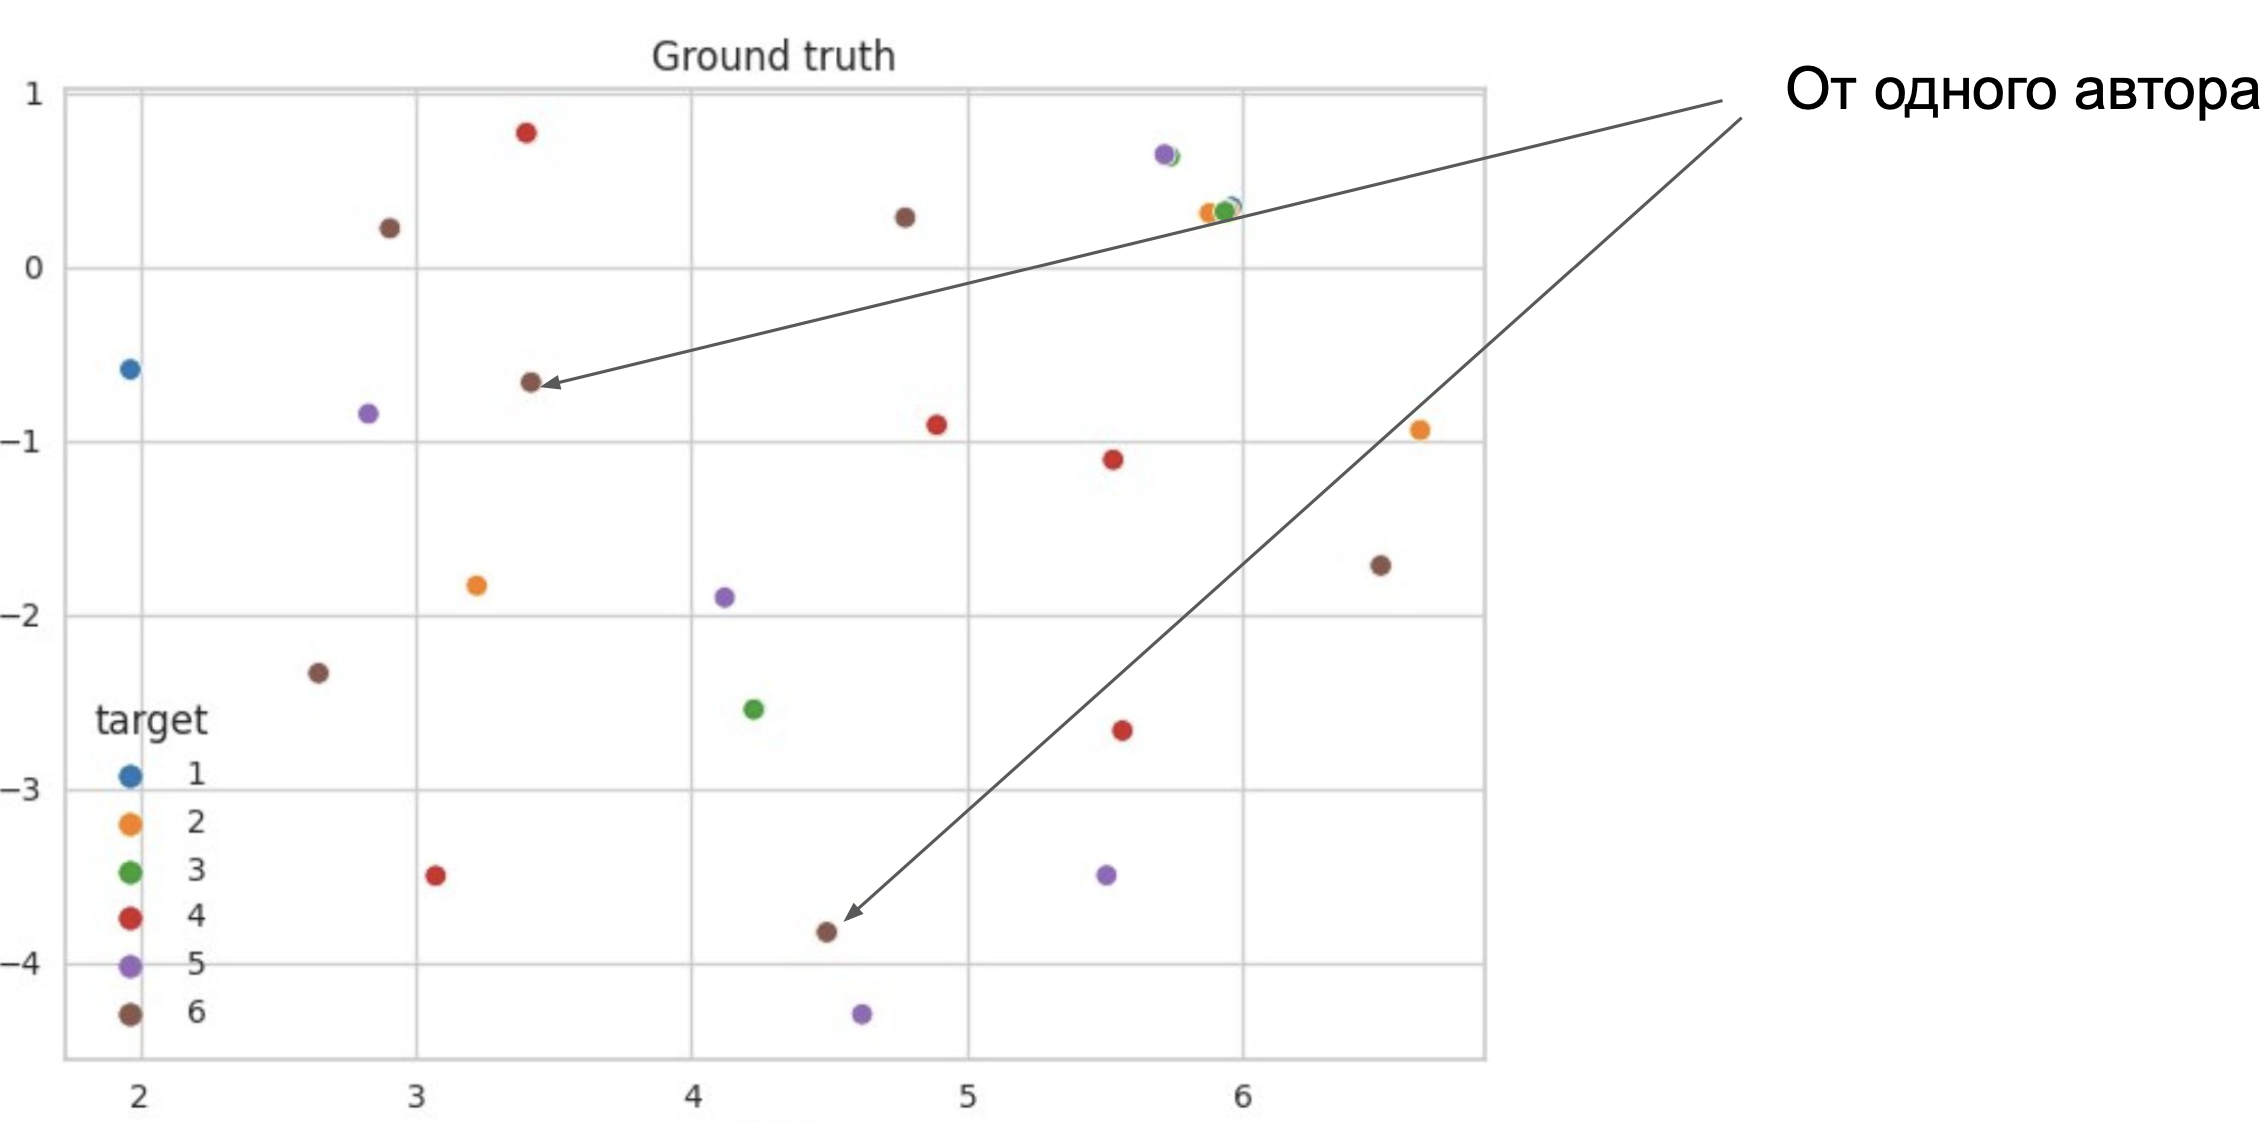
\includegraphics[width=0.9\textwidth]{8.png}
    \captionsetup{width=0.9\textwidth}
    \caption{Результат применения T-SNE к пространству эмбеддингов, полученных с помощью модели AutoEncoder + VLAD}
    \label{fig:autoencoder_result}
\end{figure}

В результате эксперимента архитектура авто-энкодера не показала должного результата. В связи с тем, что во время обучения мы никак не добивались близости эмбеддингов, который были получены из почерков от одного автора, а также из-за того, что последним слоем был VLAD, который не дает сильной гарантии кластеризуемости получаемых глобальных эмбеддингов, мы получили очень разряженное пространство векторов, которое не обладает никакими геометрическими свойствами, как показано на рисунке \ref{fig:autoencoder_result}.

\subsubsection{CVL + SNN}

% \begin{figure}[htbp]
%     \centering
%     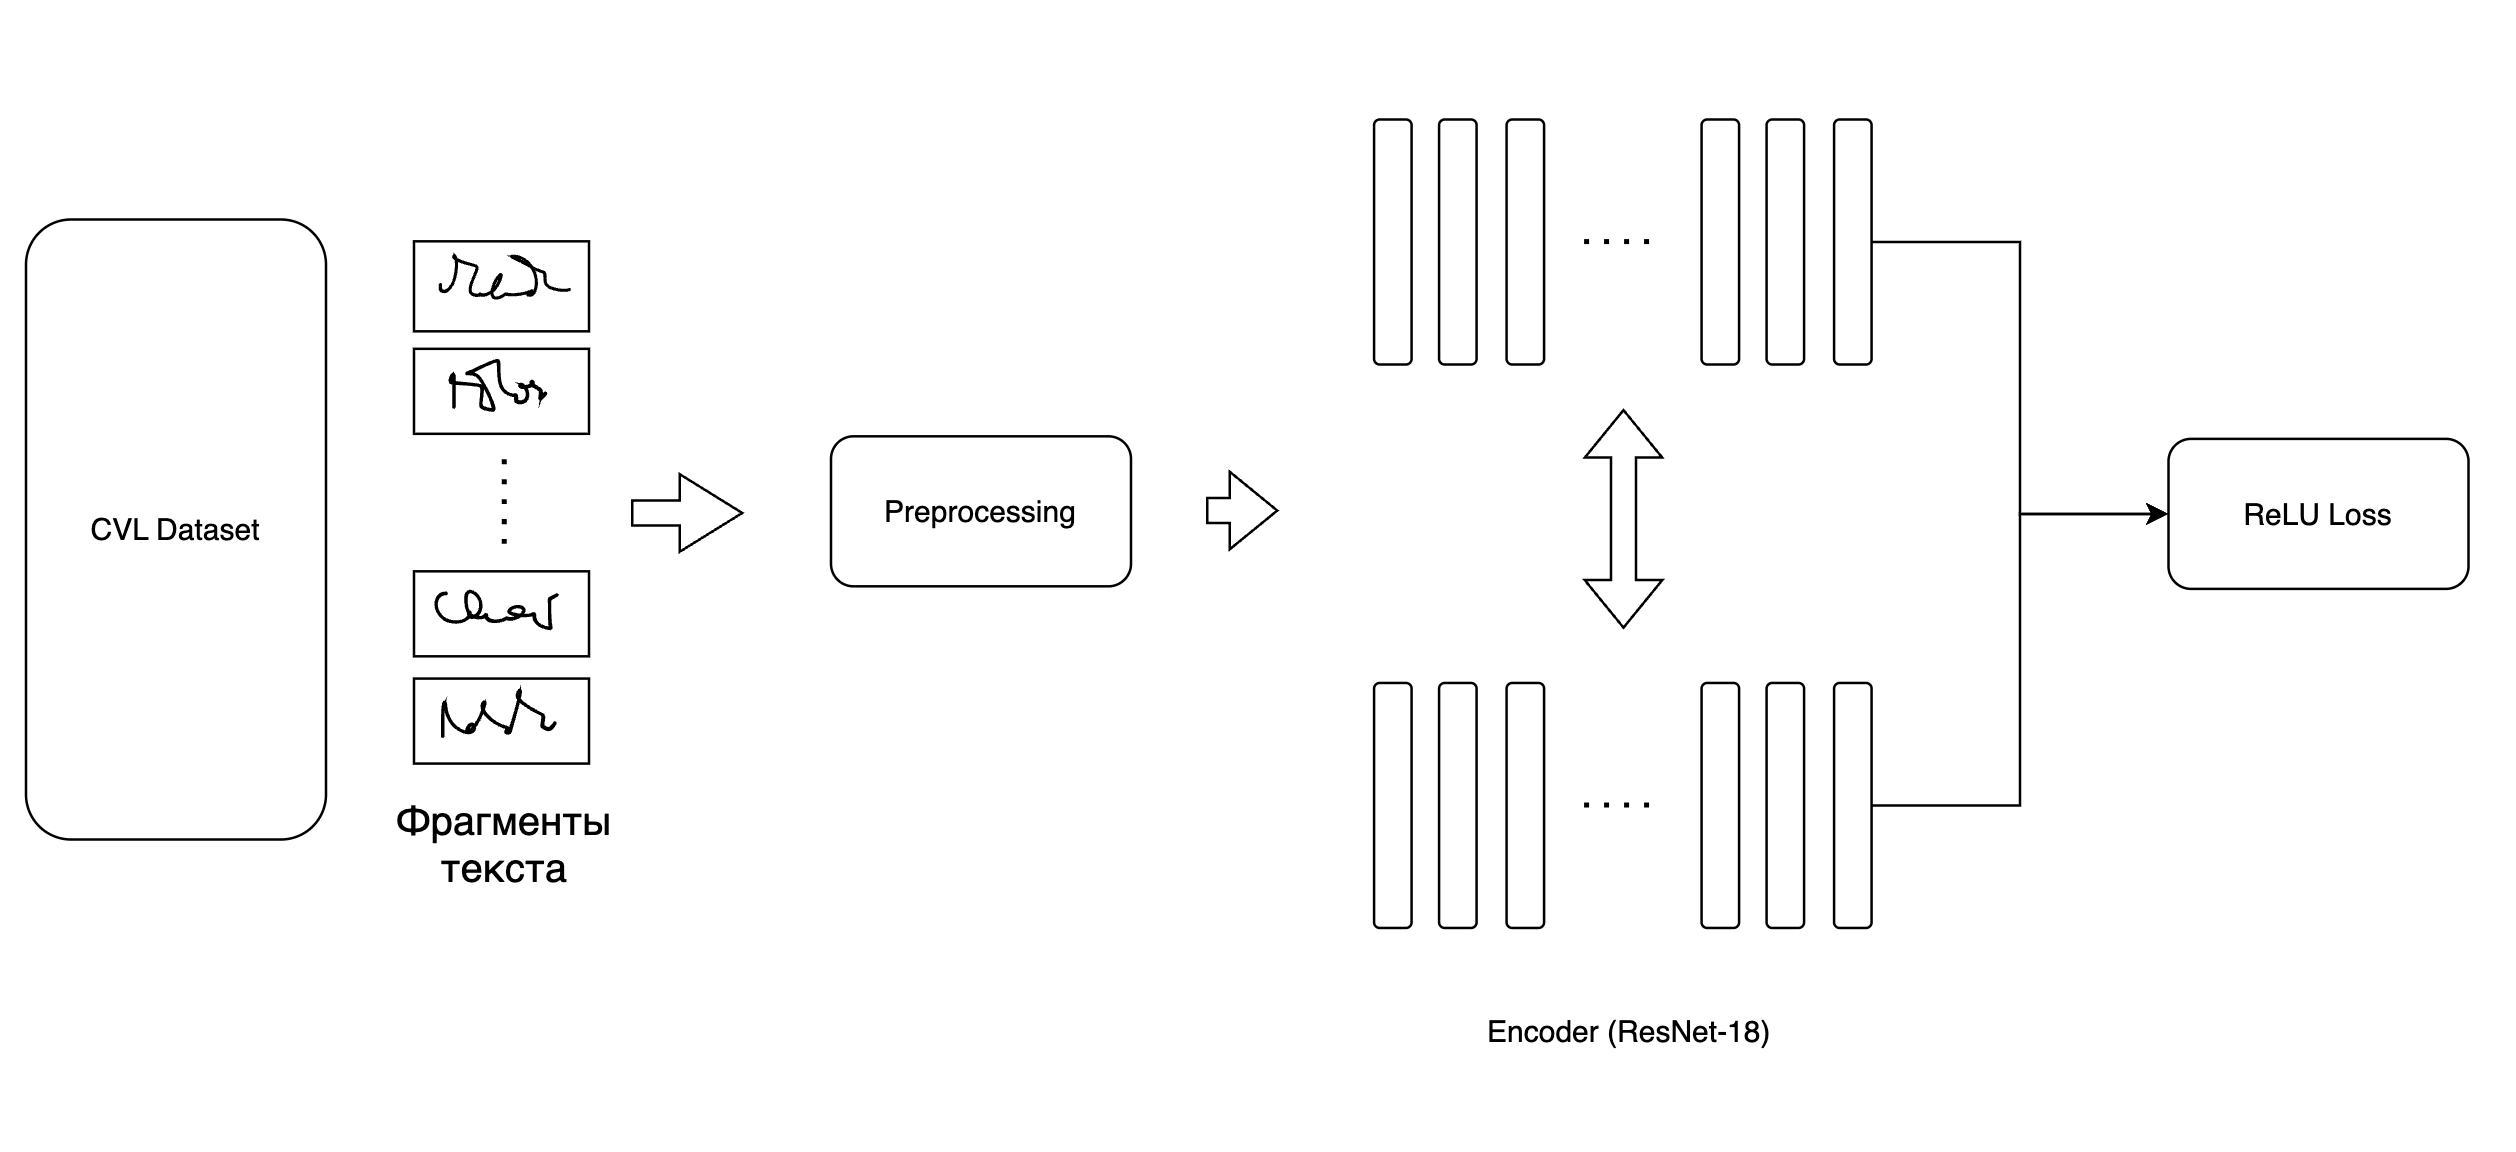
\includegraphics[width=1\textwidth]{12.png}
%     \captionsetup{width=0.9\textwidth}
%     \caption{Архитектура обучения эксперимента CVL + SNN}
%     \label{fig:snn_experiment}
% \end{figure}

Далее мы обучали модель SNN на датасете CVL. В данном эксперименте датасет никак не разбивался с помощью детектора углов. Вместо этого рукописные строчки разбивались на куски с одинаковой длиной, и определенные пары из них подавались уже самой модели. В качестве энкодера была взята модель ResNet-18, которая никак не предобучалась. Никаких агрегирований полученных эмбеддингов не производилось.

В результате обучения и прогона тестовых изображений через модель, были получены уже более репрезентативные эмбеддинги, по сравнению с предыдущей моделью. На рисунке \ref{fig:snn_experiment_2} можно видеть результат применения алгоритма T-SNE на тестовом пространстве эмбеддингов. Как мы видим, мы уже получили выделяющиеся и отдалённые друг от друга кластера. На результате применения данной модели и алгоритма кластеризации K-Means без предварительного уменьшения размерности, была вычислена метрика Cluster Accuracy, которая была равна 0.795, что говорит о неплохой кластеризуемости. Однако при увеличении количества авторов до порядка сотен, данная величина сильно упала до примерно 0.3.

\begin{figure}[htbp]
    \centering
    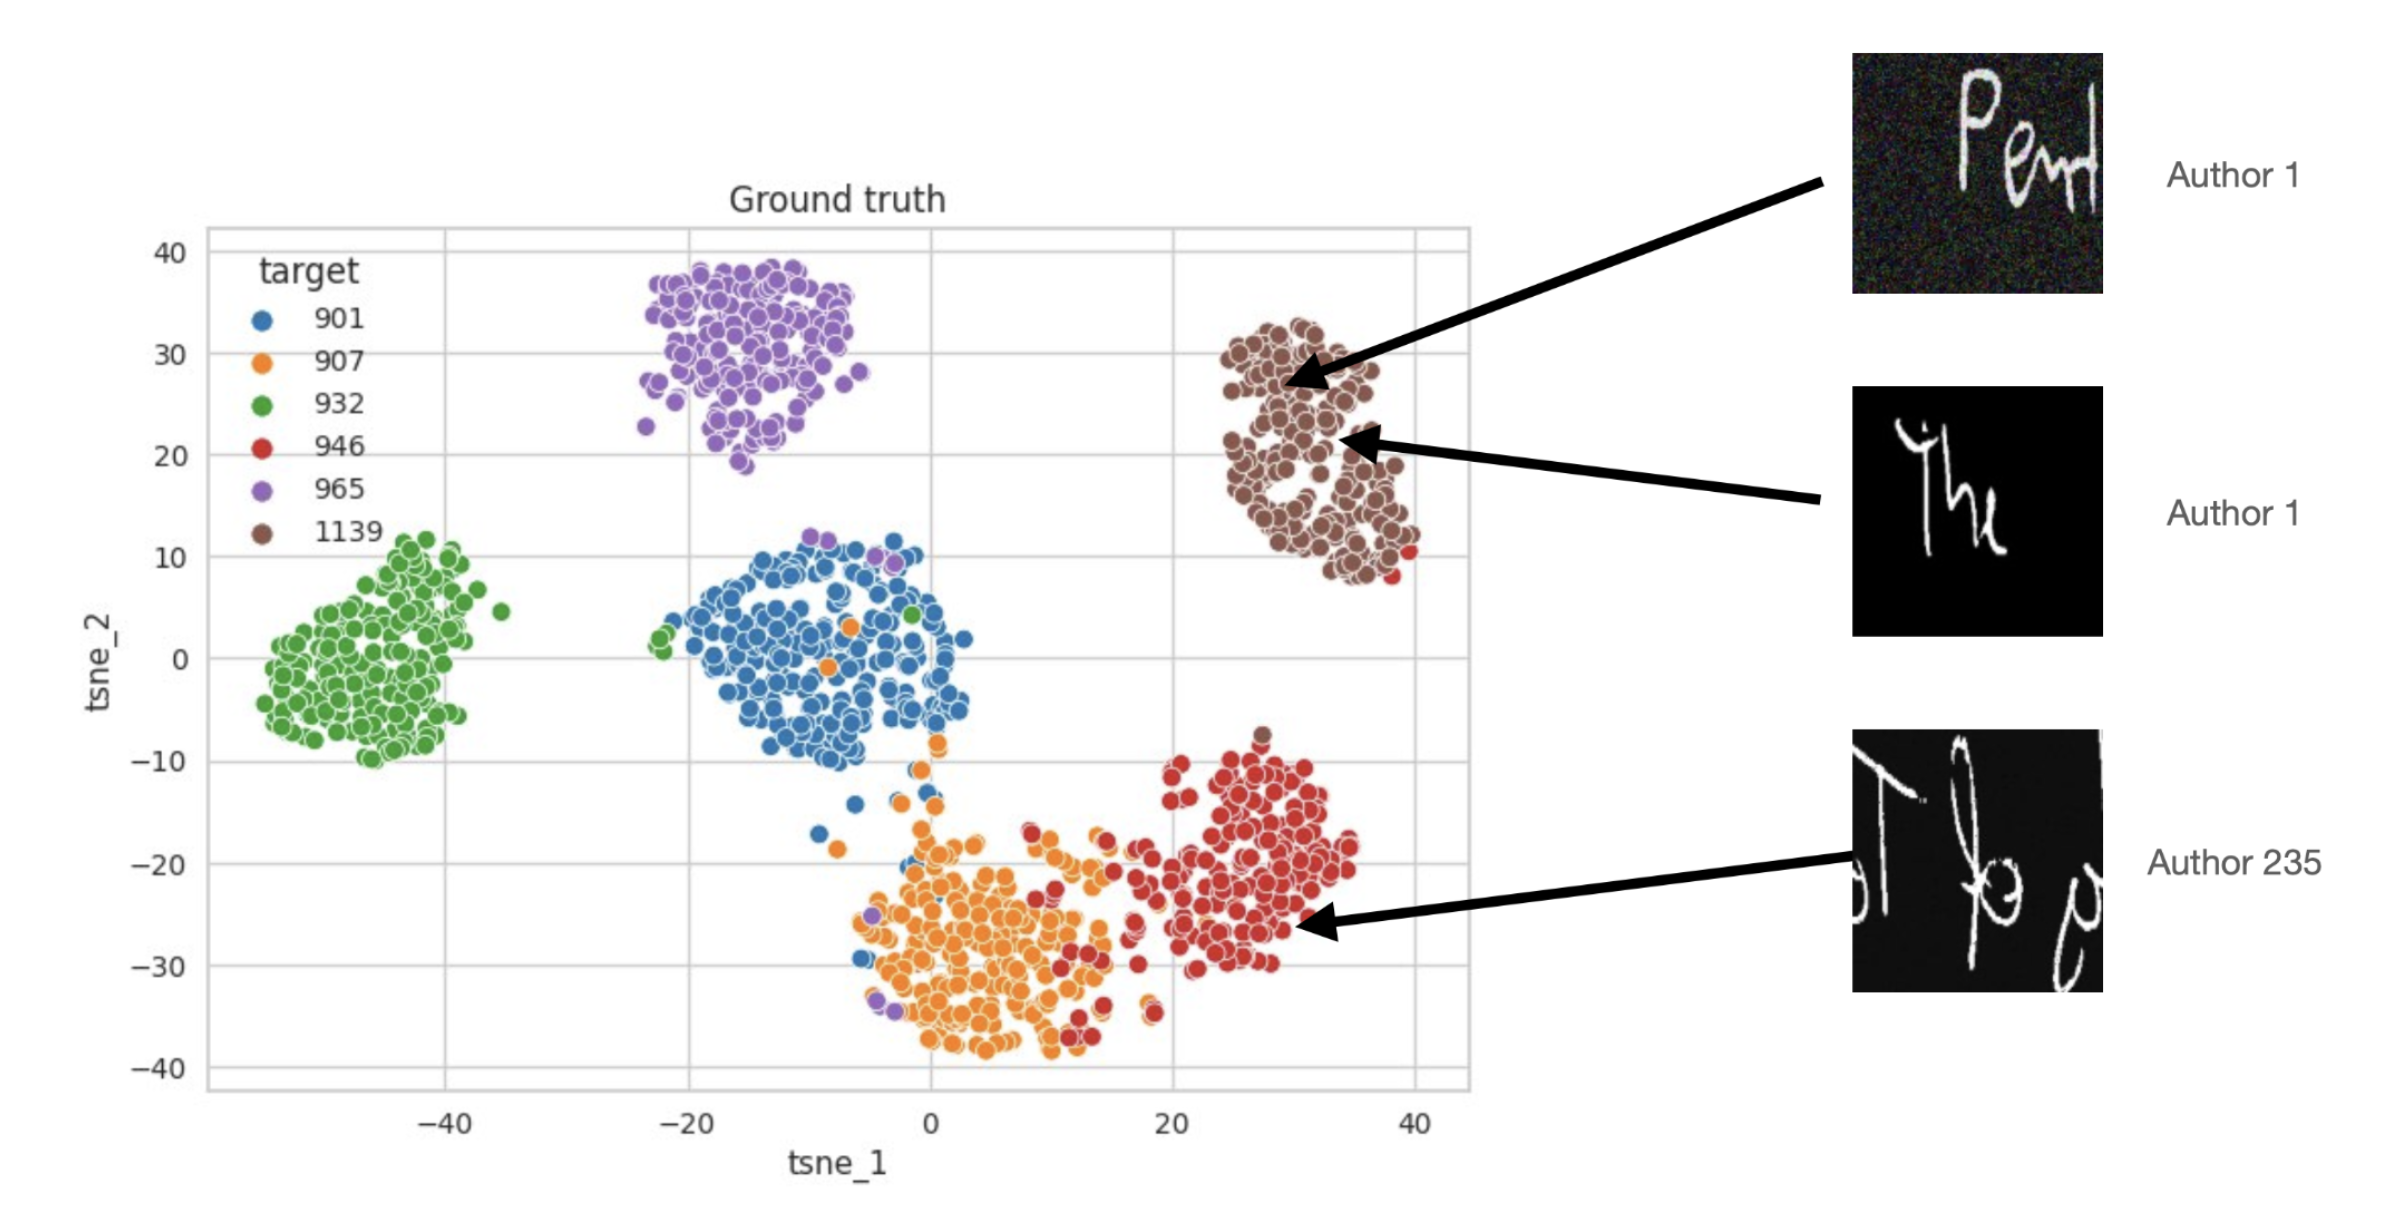
\includegraphics[width=1\textwidth]{13.png}
    \captionsetup{width=0.9\textwidth}
    \caption{Результат применения T-SNE к пространству тестовых эмбеддингов, полученных с помощью модели SNN на датасете CVL}
    \label{fig:snn_experiment_2}
\end{figure}

\subsubsection{Synthetic Dataset}

Большой проблемой при обучении модели на датасетах CVL и IAM задачи классификации был тот факт, что в общей сложности тренировочных данных было довольно мало, и модель быстро переобучалась, несмотря на применяемую аугментацию. В связи с этим было проведено обучение на упомянутом ранее синтетическом датасете, который при этом был уменьшен до 500 шрифтов. Было протестировано три конфигурации:

\begin{enumerate}
    \item Обучение на задаче классификации c функцией потерь CrossEntropy
    \item Обучение на задаче классификации с функцией потерь ArcFace
    \item Обучение сиамской архитектуры
\end{enumerate}

Данные конфигурации в связке с UMAP на этапе инференса, как указано на рисунке \ref{fig:inference}, выдавали эмбеддинги, на которых потом запускались алгоритмы кластеризации K-Means, Agglomerative Clustering и MeanShift. Также были проведены запуски с предобученным UMAP на 20\% датасета и на 0\% датасета. Тестовый датасет содержал 53 авторов из CVL, 118 авторов из IAM и 82 авторов из Synthetic.

\begin{figure}[htbp]
    \centering
    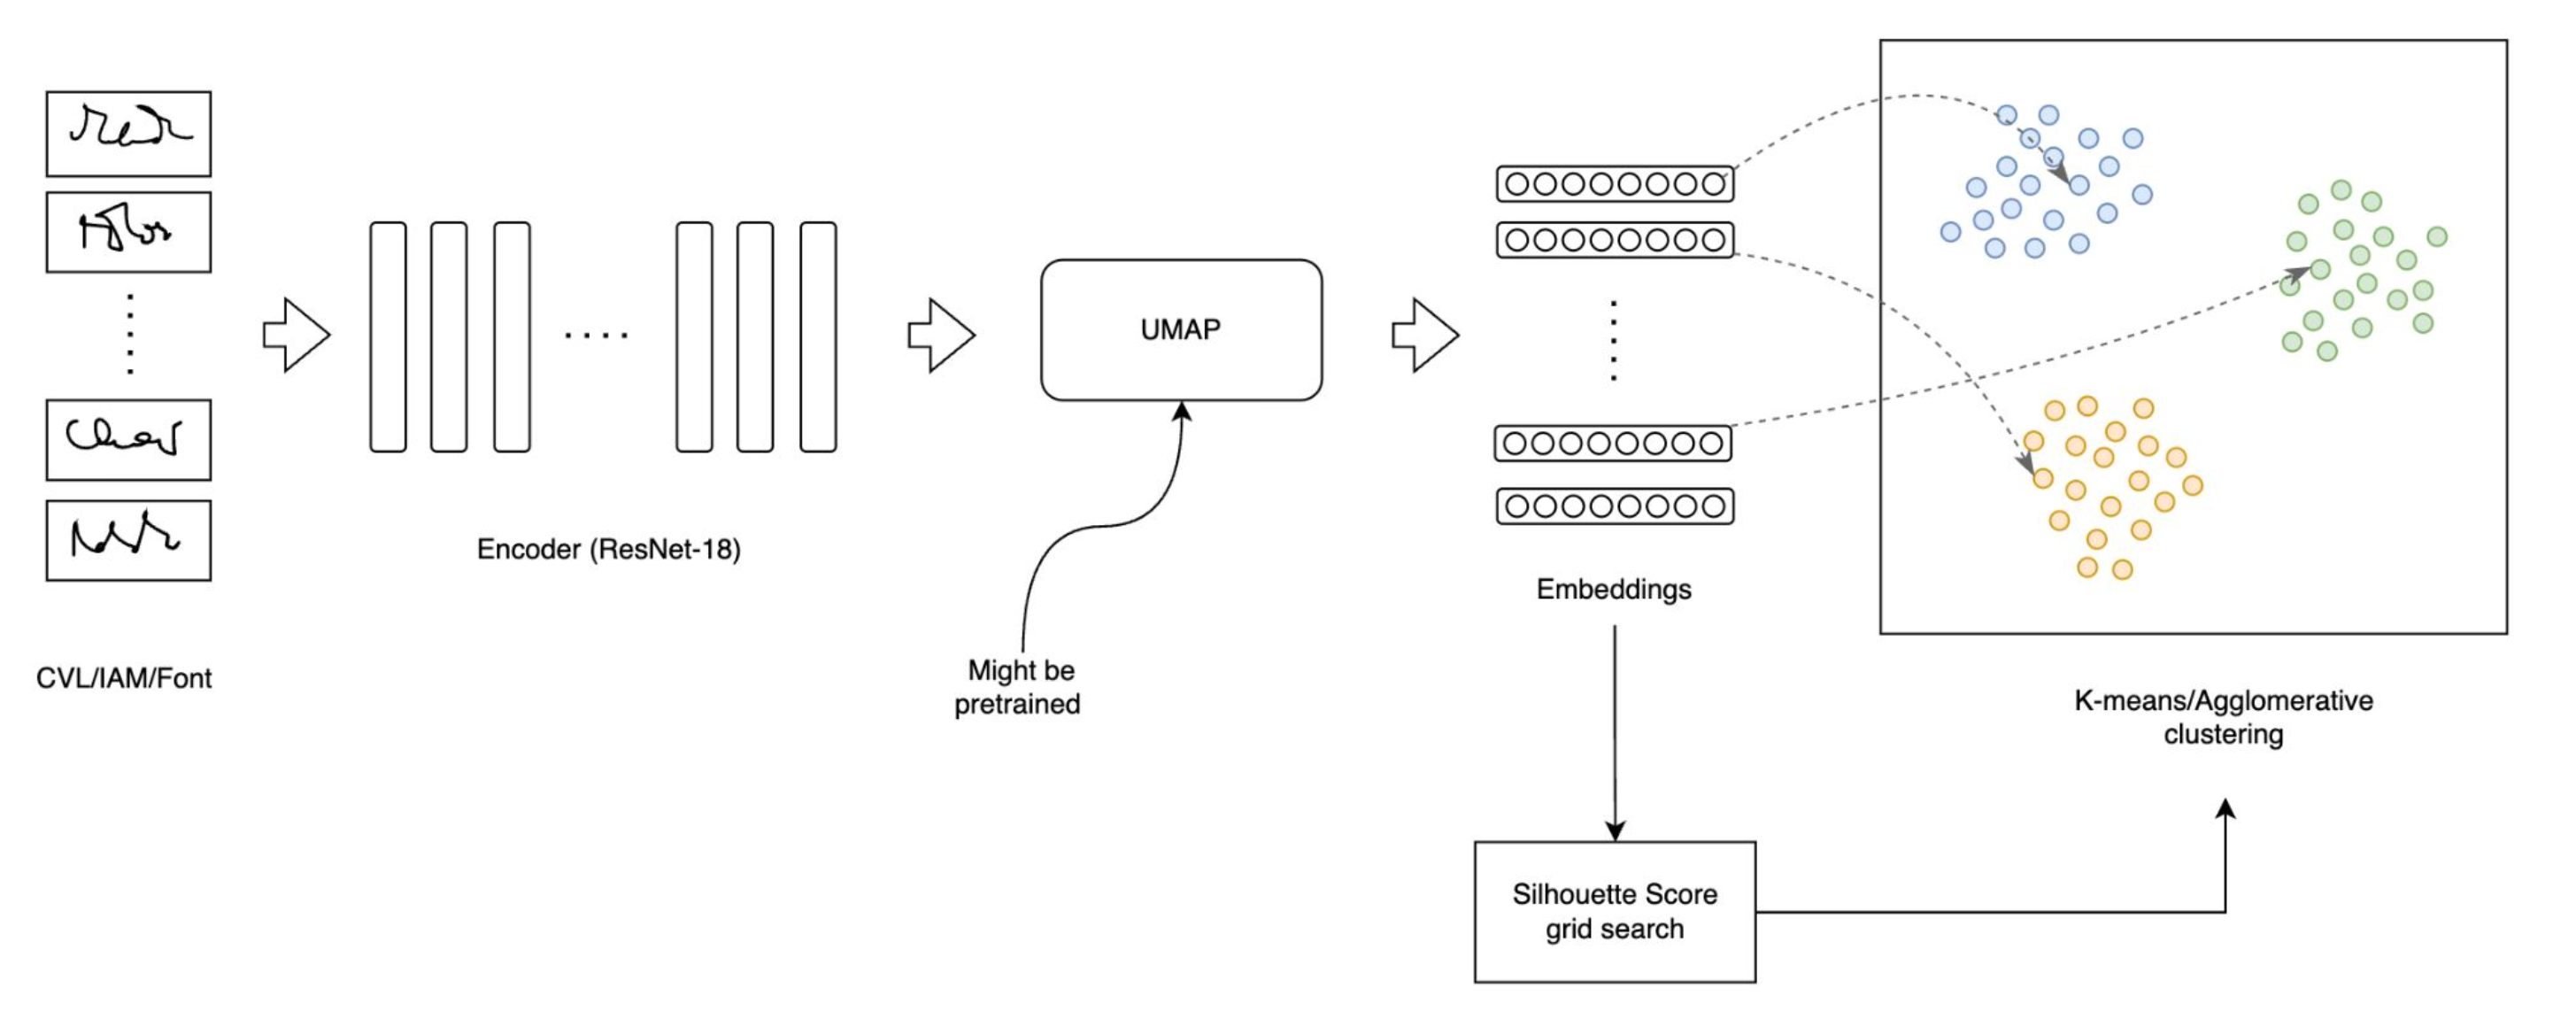
\includegraphics[width=1\textwidth]{10.png}
    \captionsetup{width=0.9\textwidth}
    \caption{Иллюстрация работы модели на этапе Inference: изображения подаются в энкодер, который выдаёт на выходе эмбеддинги. Затем эти эмбеддинги попадают в слой уменьшения размерности UMAP, который также может быть заранее предобучен на метках тренировочной выборки. Наконец, применяется алгоритм кластеризации для получения разбивки по авторам текстов}
    \label{fig:inference}
\end{figure}

Результаты экспериментов приведены в таблице \ref{table:first}. Самые лучшие показатели наблюдаются у датасета Synthetic для модели с функцией потерь Cross-Entropy. Данный результат был ожидаем, так как модель обучалась также на синтетическом датасете. Модели удалось успешно определить количество кластеров с точностью -2, и с ARI 0.85, что говорит о хорошем результате кластеризации датасета по сравнению с правильными метками. ArcFace для данного датасета не принес существенного улучшения, чего нельзя сказать о датасете IAM. Несмотря на то, что ARI для IAM хуже в случае функции потерь ArcFace, количество кластеров было определенно лучше, чем у модели с лоссом CrossEntropy. Также ArcFace дал улучшение показателей Silhouette Score для обоих датасетов.

\begin{table}[ht]
    \centering
    \captionsetup{width=0.9\textwidth}

    \hspace*{-4em}\scalebox{0.75} {
        \begin{subtable}{0.4\linewidth}
            \centering
            \caption{Silhouette Score | K-Means}
            \begin{tabular}{|c|c|c|c|}
            \hline
                & CVL & IAM & Synthetic \\
            \hline
            CE & 0.38 & 0.32 & \textbf{0.80} \\
            ArcFace & 0.53 & 0.52 & 0.75 \\
            SNN & \textbf{0.85} & 0.70 & 0.48 \\
            \hline
            \end{tabular}
        \end{subtable}

        \hfill
        \begin{subtable}{0.4\linewidth}
            \centering
            \caption{$\Delta K$ | K-Means}
            \begin{tabular}{|c|c|c|c|}
            \hline
                & CVL & IAM & Synthetic \\
            \hline
            CE & 13 & -57 & \textbf{-2} \\
            ArcFace & 28 & \textbf{-7} & 17 \\
            SNN & -33 & -68 & -43 \\
            \hline
            \end{tabular}
        \end{subtable}
        
        \hfill
        \begin{subtable}{0.4\linewidth}
            \centering
            \caption{RI / ARI | K-Means}
            \begin{tabular}{|c|c|c|c|}
            \hline
                & CVL & IAM & Synthetic \\
            \hline
            CE & 0.95/0.16 & 0.94/0.18 & \textbf{0.99/0.85} \\
            ArcFace & 0.97/0.07 & 0.94/0.06 & 0.99/0.50 \\
            SNN & 0.92/0.0005 & 0.93/0.003 & 0.95/0.000 \\
            \hline
            \end{tabular}
        \end{subtable}
    }
    \vskip 0.01\baselineskip
    \hspace*{-4em}\scalebox{0.75} {
        \begin{subtable}{0.4\linewidth}
            \centering
            \caption{Silhouette Score | Agglomerative}
            \begin{tabular}{|c|c|c|c|}
            \hline
                & CVL & IAM & Synthetic \\
            \hline
            CE & 0.31 & 0.24 & \textbf{0.78} \\
            ArcFace & 0.41 & 0.46 & 0.65 \\
            SNN & 0.65 & 0.50 & 0.38 \\
            \hline
            \end{tabular}
        \end{subtable}
    
        \hfill
        \begin{subtable}{0.4\linewidth}
            \centering
            \caption{$\Delta K$ | Agglomerative}
            \begin{tabular}{|c|c|c|c|}
            \hline
                & CVL & IAM & Synthetic \\
            \hline
            CE & 18 & -73 & \textbf{7} \\
            ArcFace & 18 & -68 & 63 \\
            SNN & -33 & -68 & -43 \\
            \hline
            \end{tabular}
        \end{subtable}
        
        \hfill
        \begin{subtable}{0.4\linewidth}
            \centering
            \caption{RI / ARI | Agglomerative}
            \begin{tabular}{|c|c|c|c|}
            \hline
                & CVL & IAM & Synthetic \\
            \hline
            CE & 0.94/0.14 & 0.93/0.16 & \textbf{0.99/0.87} \\
            ArcFace & 0.96/0.07 & \textbf{0.91/0.38} & 0.98/0.40 \\
            SNN & 0.93/0.0005 & 0.93/0.003 & 0.95/0.000 \\
            \hline
            \end{tabular}
        \end{subtable}
    }
    
    \caption{Результаты обучения: датасет Synthetic, предобучение UMAP 20\%. Результат кластеризации с помощью K-Means -- первый ряд таблиц, с помощью Agglomerative Clustering -- второй ряд. RI/ARI измерялся при предсказанном количестве кластеров, Silhouette Score -- при правильном количестве кластеров.}

    \label{table:first}
\end{table}

В случае использования алгоритма кластеризации Agglomerative, показатели для датасета Synthetic также остались хорошими. В свою очередь хорошие показатели кластеризуемости показал датасет IAM: при использовании функции потерь ArcFace значение метрики ARI выросло в чуть больше чем в два раза до 0.38, что лучше чем с использованием алгоритма K-Means для кластеризации.

Модель SNN не показала хороших результатов на всех датасетах. Несмотря на то, что показатели Silhouette Score выше, чем у остальных архитектур, значения метрики ARI близки к нулю, что говорит о том, что кластеризация почти не различима от случайного раскрашивания векторов.

Если убрать предобучение UMAP, то результаты становятся более скромными, как показано в таблице \ref{table:second}. Не смотря на то, что Silhouette Score немного вырос, Adjusted Rand Score упал почти во всех случаях, кроме синтетического датасета. Для датасета Synthetic дообучение UMAP действительно не дало сильного улучшения показателей, так как модель сама обучалась на этом огромном датасете.

Также были предприняты попытки дообучения самого энкодера на датасетах IAM/CVL после предварительного обучения на ImageNet или Synthetic. Для этого обучался совершенно новый слой классификации, при этом сам энкодер содержал старые веса, обученные на прошлых датасетах. Однако подобный эксперимент лишь ухудшил результаты.

\begin{table}[ht]
    \centering
    \captionsetup{width=0.9\textwidth}

    \hspace*{-4em}\scalebox{0.75} {
        \begin{subtable}{0.4\linewidth}
            \centering
            \caption{Silhouette Score | K-Means}
            \begin{tabular}{|c|c|c|c|}
            \hline
                & CVL & IAM & Synthetic \\
            \hline
            CE & 0.29 & 0.29 & \textbf{0.85} \\
            ArcFace & 0.55 & 0.58 & 0.75 \\
            SNN & 0.63 & 0.65 & 0.46 \\
            \hline
            \end{tabular}
        \end{subtable}

        \hfill
        \begin{subtable}{0.4\linewidth}
            \centering
            \caption{$\Delta K$ | K-Means}
            \begin{tabular}{|c|c|c|c|}
            \hline
                & CVL & IAM & Synthetic \\
            \hline
            CE & -33 & -38 & \textbf{-2} \\
            ArcFace & 73 & 23 & 42 \\
            SNN & 73 & -68 & 52 \\
            \hline
            \end{tabular}
        \end{subtable}
        
        \hfill
        \begin{subtable}{0.4\linewidth}
            \centering
            \caption{RI / ARI | K-Means}
            \begin{tabular}{|c|c|c|c|}
            \hline
                & CVL & IAM & Synthetic \\
            \hline
            CE & 0.935/0.095 & 0.94/0.12 & \textbf{0.99/0.90} \\
            ArcFace & 0.97/0.05 & 0.94/0.06 & 0.99/0.51 \\
            SNN & 0.97/0.003 & 0.93/0.005 & 0.98/0.000 \\
            \hline
            \end{tabular}
        \end{subtable}
    }
    \vskip 0.01\baselineskip
    \hspace*{-4em}\scalebox{0.75} {
        \begin{subtable}{0.4\linewidth}
            \centering
            \caption{Silhouette Score | Agglomerative}
            \begin{tabular}{|c|c|c|c|}
            \hline
                & CVL & IAM & Synthetic \\
            \hline
            CE & 0.23 & 0.24 & \textbf{0.84} \\
            ArcFace & 0.47 & 0.53 & 0.73 \\
            SNN & 0.64 & 0.65 & 0.45 \\
            \hline
            \end{tabular}
        \end{subtable}
    
        \hfill
        \begin{subtable}{0.4\linewidth}
            \centering
            \caption{$\Delta K$ | Agglomerative}
            \begin{tabular}{|c|c|c|c|}
            \hline
                & CVL & IAM & Synthetic \\
            \hline
            CE & 43 & -38 & \textbf{-1} \\
            ArcFace & 73 & 62 & 52 \\
            SNN & 73 & -68 & 72 \\
            \hline
            \end{tabular}
        \end{subtable}
        
        \hfill
        \begin{subtable}{0.4\linewidth}
            \centering
            \caption{RI / ARI | Agglomerative}
            \begin{tabular}{|c|c|c|c|}
            \hline
                & CVL & IAM & Synthetic \\
            \hline
            CE & 0.94/0.13 & 0.93/0.11 & \textbf{0.99/0.9} \\
            ArcFace & 0.96/0.05 & 0.94/0.12 & 0.99/0.53 \\
            SNN & 0.965/0.003 & 0.93/0.004 & 0.98/0.000 \\
            \hline
            \end{tabular}
        \end{subtable}
    }
    
    \caption{Результаты обучения: датасет Synthetic, предобучение UMAP 0\%. Расположение таблиц аналогично таблице \ref{table:first}.}

    \label{table:second}
\end{table}

\begin{figure}[htbp]
    \centering
    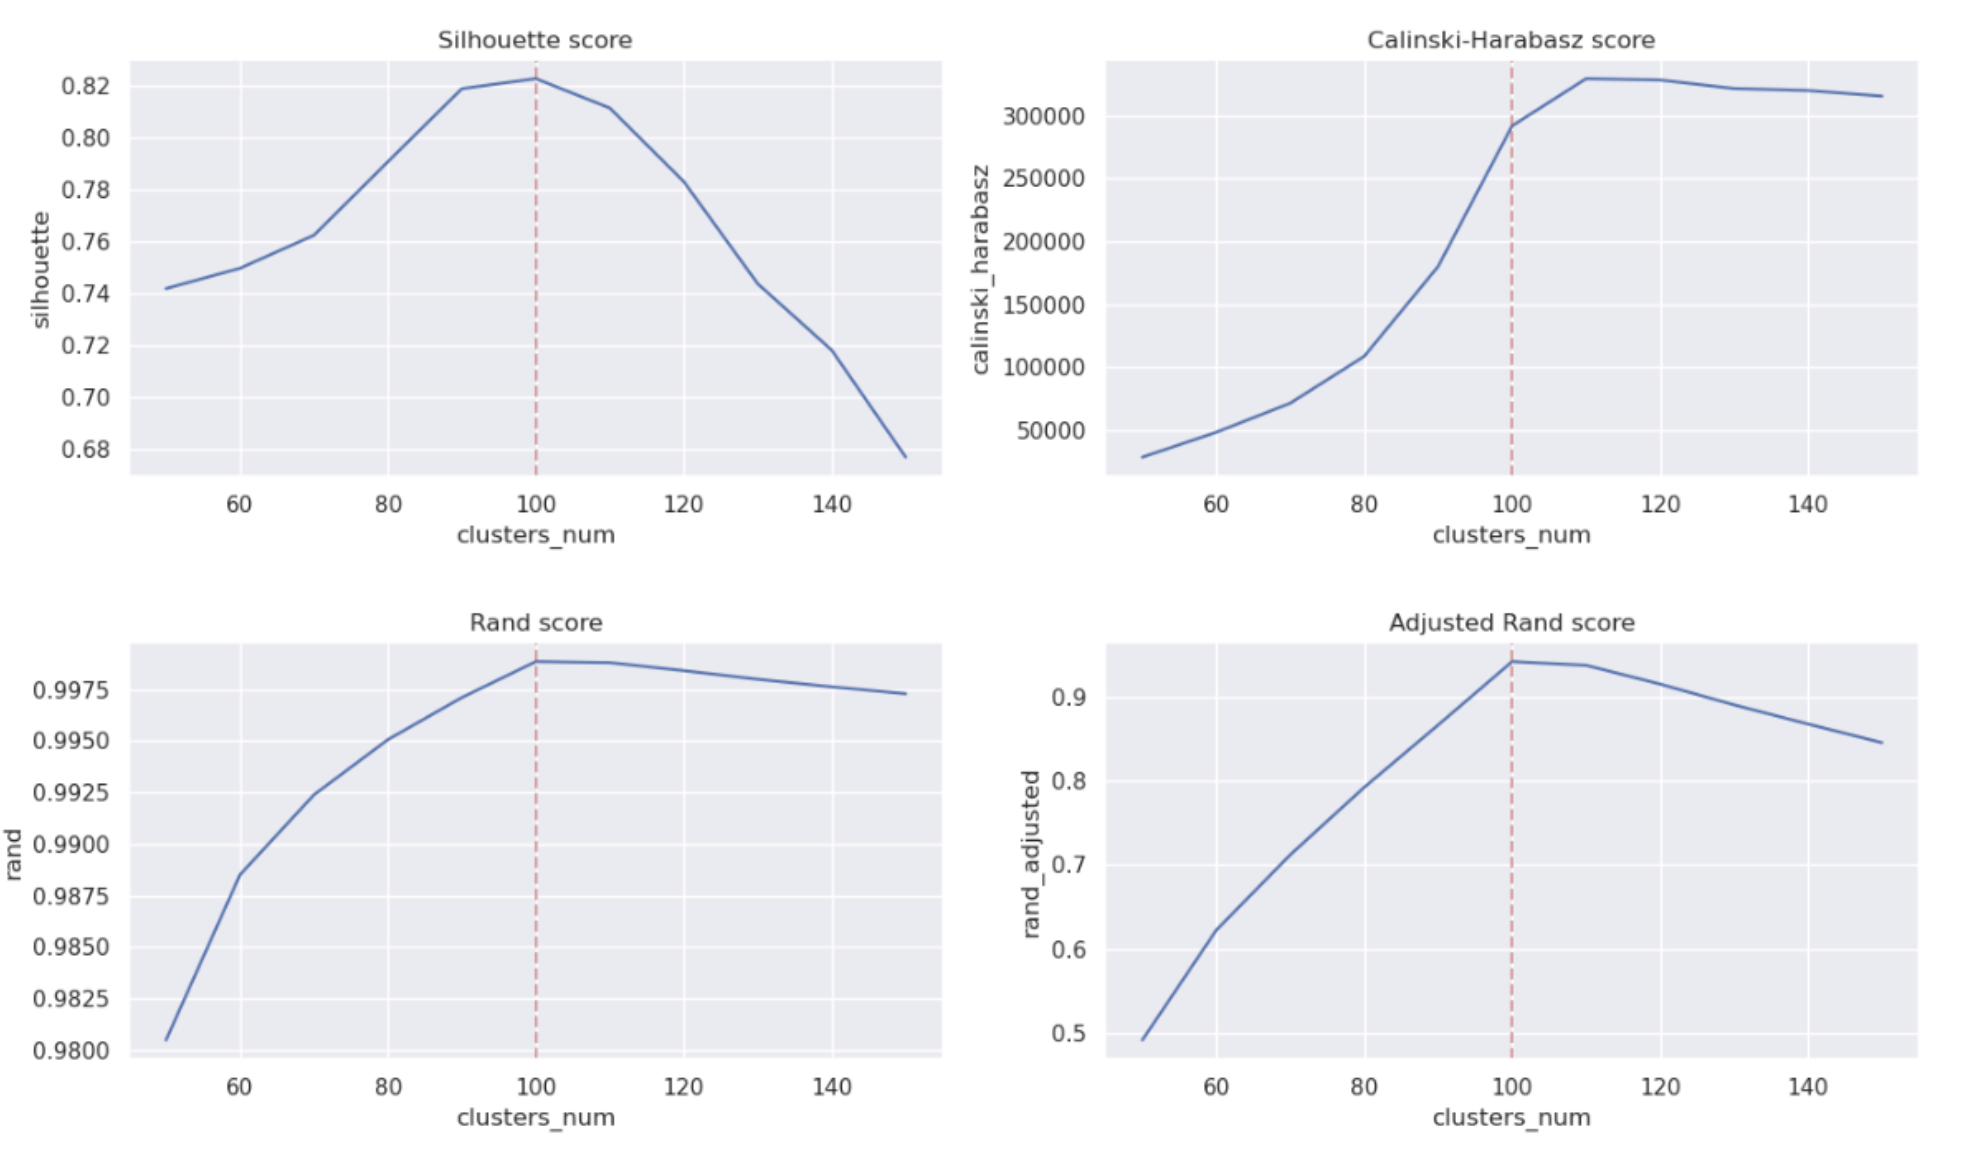
\includegraphics[width=1\textwidth]{15.png}
    \captionsetup{width=0.9\textwidth}
    \caption{Изменение различных метрик в зависимости от выбранного количества кластеров на примере датасета Synthetic. Правильное количество кластеров отмечено красной прямой по оси абсцисс.}
    \label{fig:synthetic_plots}
\end{figure}

\clearpage

Пример выполнения поиска количества кластеров по сетке можно видеть на рисунке \ref{fig:synthetic_plots}. Silhouette score сначала растет по направлению к правильному количеству кластеров, а затем убывает, что является индикатором того, что пространство векторов хорошо кластеризуемо. Это и подтверждают supervised метрики RI и ARI, которые ведут себя точно также. Также можно заметить, что индикатор Calinski-Harabasz не является репрезентативным, так как правильное количество кластеров, отмеченное красной прямой, не попадает в максимум визуально. При этом мы можем наблюдать, что Silhouette Score достигает максимума именно при правильном количестве кластеров, что говорит о том, что он является хорошим индикатором для поиска данного параметра. 


\subsubsection{IAM + NetVLAD + TripletLoss}

\begin{figure}[htbp]
    \centering
    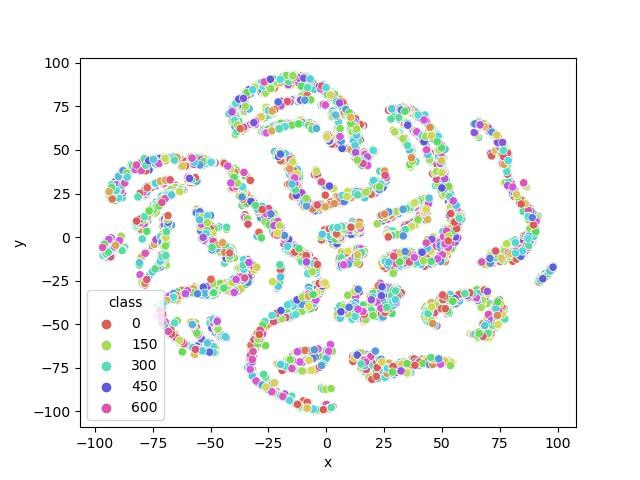
\includegraphics[width=0.8\textwidth]{16.jpg}
    \captionsetup{width=0.9\textwidth}
    \caption{Результат применения T-SNE к результату модели NetVLAD + TripletLoss на тестовом датасете.}
    \label{fig:triplet}
\end{figure}

\begin{table}[ht]
    \centering
    \captionsetup{width=0.9\textwidth}

    \hspace*{-4em}\scalebox{0.9} {
        \begin{subtable}{0.5\linewidth}
            \centering
            \caption{Silhouette Score}
            \begin{tabular}{|c|c|c|c|}
            \hline
                & CVL & IAM & Synthetic \\
            \hline
            KMeans & 0.74 & 0.47 & 0.48 \\
            Agglomerative & 0.75 & 0.48 & 0.46 \\
            \hline
            \end{tabular}
        \end{subtable}

        \hfill
        \begin{subtable}{0.5\linewidth}
            \centering
            \caption{$\Delta K$}
            \begin{tabular}{|c|c|c|c|}
            \hline
                & CVL & IAM & Synthetic \\
            \hline
            KMeans & -33 & -68 & -42 \\
            Agglomerative & -33 & -68 & -42 \\
            \hline
            \end{tabular}
        \end{subtable}
    }

    \vskip 0.01\baselineskip
    \hspace*{-4em}\scalebox{0.9} {
        \begin{subtable}{0.5\linewidth}
            \centering
            \caption{RI / ARI}
            \begin{tabular}{|c|c|c|c|}
            \hline
                & CVL & IAM & Synthetic \\
            \hline
            KMeans & 0.78/0.017 & 0.01/0.00 & 0.97/0.04 \\
            Agglomerative & 0.78/0.018 & 0.01/0.00 & 0.98/0.04 \\
            \hline
            \end{tabular}
        \end{subtable}
    }
    
    \caption{Результаты обучения NetVLAD + TripletLoss: датасет IAM, предобучение UMAP 0\%.}

    \label{table:third}
\end{table}


В данном эксперименте обучалась модель ResNet-18 с конечным слоем в виде связки NetVLAD и TripletLoss, аналогично работе \cite{netvlad}. Модель обучалась на датасете IAM, причем сам энкодер был предобучен на ImageNet, чтобы нивелировать шанс переобучения. Пайплайн для инференса выглядел похожим образом, как и в предыдущем эксперименте (рис \ref{fig:inference}). 

В результате эксперимента результаты \ref{table:third} оказались хуже эксперимента с синтетическим датасетом. Triplet loss не смог создать во время обучения кластеризуемые эмбеддинги, что можно увидеть на иллюстрации \ref{fig:triplet}. В результате прогона через модель вырисовываются кластера, но общее множество авторов смешивается на одном вытянутом "острове".

Также показатели вышеописанных метрик показывают, что кластеризация проходит хуже. Не смотря на то, что Silhouette Score возрос для датасета CVL и IAM, показатели ARI для датасета IAM, на котором обучалась сеть, близки к нулю, что говорит о раскраске, близкой к случайной. 

\newpage 
\newpage
\section{Заключение}

Был проведён обзор существующих технологий решения задачи классификаций авторов по рукописному тексту, а также других проблем компьютерного зрения. В результате этого было проведено несколько экспериментов, которые заключались в объединении нескольких вышеупомянутых идей для решения поставленной задачи. После проведения экспериментов можно сделать следующие выводы:

\begin{enumerate}
    \item Модель обученная на архитектуре AutoEncoder не смогла показать должного результата в следствии того, что в неё саму закладывается слишком много ожиданий от выходных геометрических свойств пространства эмбеддингов.
    \item Сиамская нейронная сеть показала хороший результат кластеризации на малом количестве авторов. При увеличении количества писателей точность решения задачи сильно снижается.
    \item Идея синтетического датасета позволила увеличить размер тренировочного датасета в десятки раз, что положительно повлияло на результаты обучения глубоких свёрточных нейронных сетей на задаче классификации. При этом искусственный датасет не мог предоставить достаточной вариативности, чтобы быть максимально похожим на человеческий почерк, что было отражено в результатах эксперимента.
    \item Алгоритм UMAP является универсальным способом уменьшения размерности пространства эмбеддингов. Обладая большим количеством параметров, он способен не только уменьшать размерность, сохраняя геометрические свойства изначального пространства, но делать его более кластеризуемым. Более того, способность частично обучиться на подаваемом датасете позволяет еще больше улучшить результаты.
    \item Архитектура обучения на задаче классификации с функцией потерь CrossEntropy имеет хорошие показатели кластеризации для синтетического датасета.
    \item Функция потерь ArcFace позволила улучшить результаты по некоторым параметрам кластеризации благодаря иной идее расположения векторов в пространстве при обучении сети.
    \item VLAD и NetVLAD в связке с архитектурой AutoEncoder и функцией потерь TripletLoss не смогли дать ожидаемого результата кластеризации. Эмбеддинги либо были равномерно раскиданы по все пространству, либо кластеризовались в "острова", в которых содержались разные авторы.
\end{enumerate}
